\documentclass{article}

%% libraries 
\usepackage{array}
\usepackage[utf8]{inputenc}
\usepackage{listings}
\usepackage{fancyhdr}
\usepackage{lastpage}
\usepackage{float}
\usepackage{url}
\usepackage{xcolor}
\usepackage{hyperref}
\usepackage{nameref}
\usepackage{enumitem}
\usepackage{adjustbox}
\usepackage{amssymb}
\usepackage{amsthm}
\usepackage{amsmath}
\usepackage{mathtools}
\usepackage{algorithm}
\usepackage{algpseudocode}
\usepackage{algcompatible}
\usepackage[numbers,sort&compress]{natbib}
\usepackage{tikz}
\usepackage{pgfplots}
\usepackage{textcomp}
\usepackage{subcaption}
\usepackage{fontawesome5}
\usepackage{tabularx}
\usepackage{multirow}
\usepackage{booktabs}
\usepackage{longtable}
\usepackage{lscape}
\usepackage{svg}
\usepackage[none]{hyphenat}

\graphicspath{{../../notebooks/figures/}}

%% doc settings
\hyphenchar\font=-1 % suppress hyphenation
\setlength\parindent{0pt} % suppress indentation
\setlength{\parskip}{0.75em} % separate paragraphs
\usepackage[margin=1.2truein]{geometry} % set page margins
\renewcommand{\tabularxcolumn}[1]{m{#1}} % left-justified
\sloppy

%% suppress section numbers
\makeatletter
\renewcommand{\@seccntformat}[1]{}
\makeatother

%% link viz
\hypersetup{
    colorlinks=true,
    linkcolor=red,
    urlcolor=red,
    citecolor=red
}

%% figs
\usetikzlibrary{
    shapes,
    arrows,
    arrows.meta,
    positioning,
    backgrounds,
    shapes.multipart,
    calc
}

\tikzset{
    block/.style={draw, fill=white, rectangle, minimum height=48pt, minimum width=48pt},
    round/.style={draw, fill=white, circle},
    sum/.style={draw, fill=white, circle, node distance=2cm},
    input/.style={coordinate},
    output/.style={coordinate},
}

\pgfplotsset{compat=newest}

%% code colors 
\definecolor{codegreen}{rgb}{0,0.6,0}
\definecolor{codegray}{rgb}{0.5,0.5,0.5}
\definecolor{codepurple}{rgb}{0.58,0,0.82}
\definecolor{backcolour}{rgb}{0.95,0.95,0.92}

\lstdefinelanguage{python}{
    % backgroundcolor=\color{backcolour},   
    % commentstyle=\color{codegreen},
    % keywordstyle=\color{blue},
    % numberstyle=\tiny\color{codegray},
    % stringstyle=\color{codepurple},
    basicstyle=\ttfamily\footnotesize,
    % breakatwhitespace=false,         
    breaklines=true,                 
    captionpos=b,                    
    % keepspaces=true,                 
    % numbers=left,                    
    % numbersep=5pt,                  
    % showspaces=false,                
    % showstringspaces=false,
    % showtabs=false,                  
    tabsize=2
}

\lstdefinelanguage{json}{
    basicstyle=\ttfamily\footnotesize,
    showstringspaces=false,
    keywordstyle=\color{blue},
    stringstyle=\color{black},
    string=[s]{"}{"}
}

\lstdefinestyle{sql}{
    language=SQL,
    basicstyle=\ttfamily\footnotesize,
    keywordstyle=\color{blue}\bfseries,
    identifierstyle=\color{black},
    stringstyle=\color{red},
    commentstyle=\color{green},
    morecomment=[l]{--},
    morecomment=[s]{/*}{*/}
}

%% math ops
\DeclareMathOperator*{\argmax}{argmax}

%% algo comments
\renewcommand{\algorithmiccomment}[1]{\texttt{//#1}}

%% page nums
\pagestyle{fancy}
\fancyhf{}
\fancyfoot[C]{Pg. \thepage \space of \pageref*{LastPage}}
\renewcommand{\headrulewidth}{0pt}

%% begin doc
\begin{document}
\title{A General Capacity Frontier of Complex Networks}
\author{
    Nicholas Kunz \href{mailto:nhk37@cornell.edu}{nhk37@cornell.edu}\\
    H. Oliver Gao \href{mailto:hg55@cornell.edu}{hg55@cornell.edu}\\~\\
    Systems Engineering, Cornell University}
\date{\today}
\maketitle

%% abstract
\begin{abstract}
\noindent
    From cells to cities, ecosystems to economies, complex networks exhibit peak intensities that define their empirical limit. Estimating these limits traditionally requires domain-specific knowledge. We demonstrate that a wide range of complex networks share a capacity frontier that constrains these maxima. We formalize this regularity by proposing Structural Capacity Theory for Network Substrate Structured Systems. These systems couple a fixed network substrate with an observable dynamical process. The frontier is learned from a vector representation of the network substrate and modulated log-additively by a vector representation of the dynamical process. Frontiers trained on one set of domains reliably bound empirical maxima of entirely different ones without observing their peak intensities or simulating their dynamics. Independent learning paradigms converge on consistent upper bounds. Frontier performance is stable under perturbation, yet degrades under deliberate falsification, with no performance gain under ablation. These findings support the capacity frontier as a generalizable constraint that describes how network structure bounds dynamical processes across otherwise unrelated systems.
\end{abstract}

%% untitled intro
\vspace{1em}
\phantomsection
\label{sec:intro}
Maxima are critical for understanding complex networks. They are important because maxima are boundary characteristics where critical thresholds are met that mark changes in network behavior \citep{ref01, ref02, ref16, ref33, ref34}. For example, a regulatory network that exceeds its threshold of localized molecular activity changes regimes \citep{ref25,ref02}. A transportation network that exceeds its carrying capacity changes behavior primarily by congestion, not by design \citep{ref03,ref04}. It is known that maxima can affect network behavior, but examining \textit{how} is traditionally understood using domain-specific interpretations \citep{ref02,ref03}. It is unclear whether network maxima express a common regularity across domains \citep{ref13,ref14,ref15}. Addressing this question requires a shared basis of comparison.

In the previous examples, network structure formed the basis on which a dynamical process occurred \citep{ref02, ref03, ref04, ref05, ref15, ref33}. Size, connectivity, spectral organization, and other topological characteristics constrain network throughput, propagation, and synchronization \citep{ref07,ref08,ref28,ref35,ref09,ref30,ref10,ref11,ref27,ref32}. The same network substrate can have different limits depending on the observational definition, activity attribution, temporal aggregation, and measurement regime \citep{ref06,ref26,ref12}. Conversely, structurally distinct substrates and dynamical processes can exhibit comparable limits under shared measurement conventions and operational definitions \citep{ref17,ref18,ref15}. In both cases, empirical maxima reflect the network substrate and the dynamical process by which observations are attributed, generated, and measured.

%% fig 1
\begin{figure}[H]
\centering
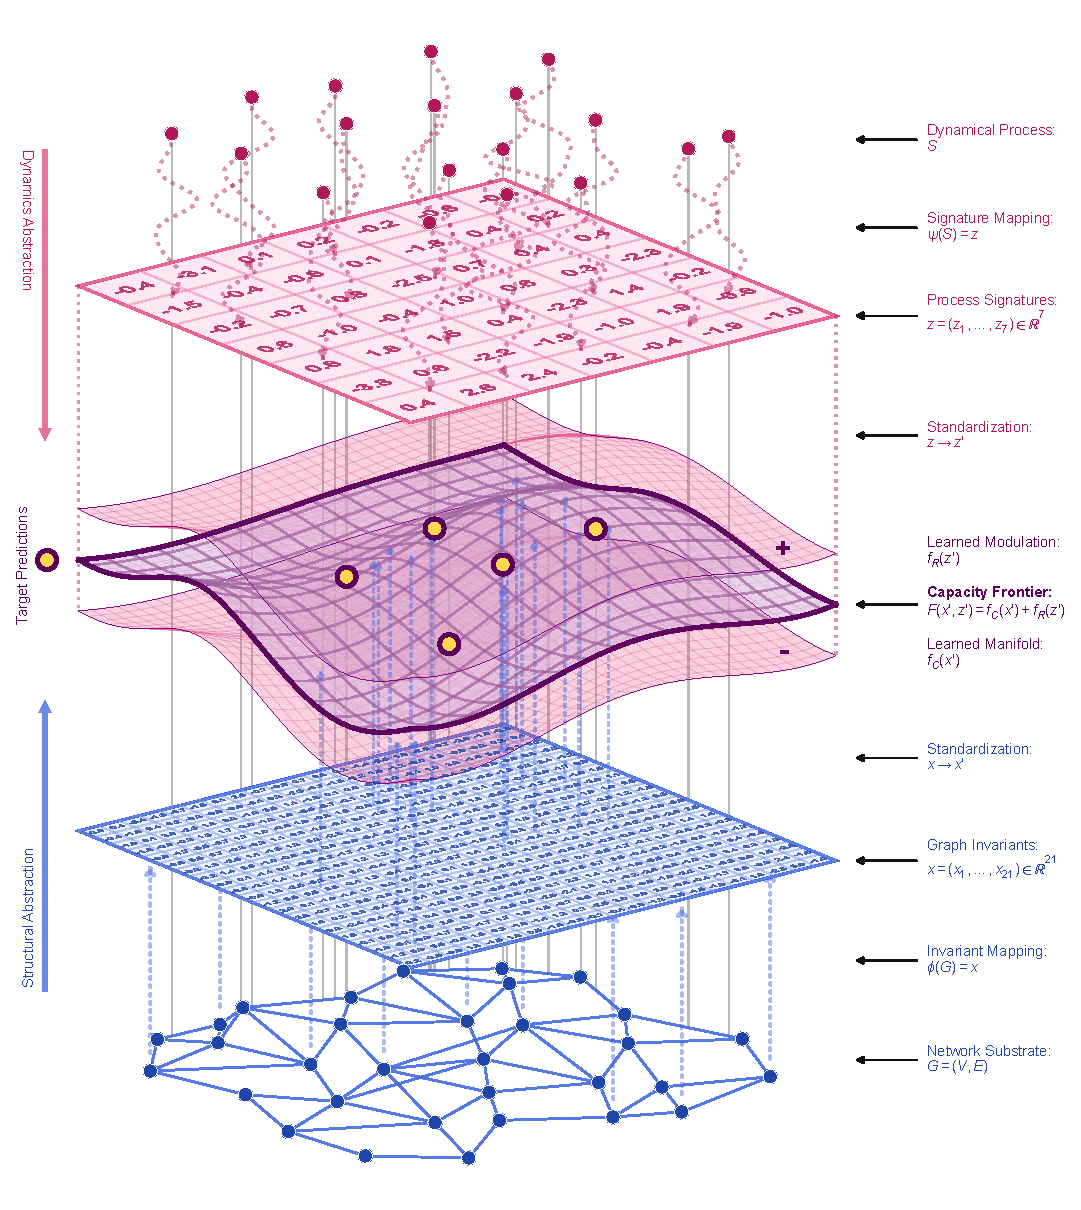
\includegraphics[width=\linewidth]{fig1.pdf}
\caption{
    \textbf{Conceptual representation of Structural Capacity Theory (SCT).} Schematic overview of the Network Substrate Structured Systems (N3S) framework as it relates to the capacity frontier. The network substrate $G$ (blue graph on bottom) is encoded as a standardized graph invariant vector $x'$ on the structural plane. The dynamical process $S$ (pink markers on top) produces observations attributed to substrate elements and is encoded as a standardized process signature vector $z'$ on the dynamics plane. The curved manifold represents the capacity frontier $F(x', z') = f_C(x') + f_R(z')$, where the fitted structural component $f_C(x')$ is modulated log-additively by the fitted process component $f_R(z')$ to estimate an upper envelope of empirical maxima $y^*$ (gold points in center).
}
\label{fig:concept}
\end{figure}
\clearpage

We propose Network Substrate Structured Systems (N3S) as a class of systems for which this coupling can be assessed. An N3S is defined by a fixed network substrate, an observable dynamical process that corresponds to that substrate, and a measurable maximum that corresponds to that dynamical process (Fig.~\ref{fig:concept}). Membership is determined from the observations a given system naturally provides so that the scope of the theory is fixed before it is tested. Structural Capacity Theory (SCT) proposes that empirical maxima from \textit{any} N3S are comparable when represented in a shared coordinate system, and that within that representation, maxima are constrained by a common capacity frontier.

We estimate the capacity frontier as a covariate-dependent upper envelope. Typical network activity can be captured by a conditional mean, but the quantity of interest is the ceiling, so the estimators are trained as such \citep{ref19,ref20,ref21,ref22,ref23,ref31,ref29}. The system's network structure and dynamical process are encoded as standardized vector representations $x'$ and $z'$, respectively. The capacity frontier $F(x', z') = f_C(x') + f_R(z')$ log-additively bounds the log-transformed maximum $y^* = \ln(1 + r_{\max})$. The frontier is strictly empirical. It permits a small fraction of observations to cross it and carries no claim of analytical containment.

We evaluate whether this formulation supports a transferable, consistent, stable, falsifiable, and decomposable capacity frontier. We found a frontier that bounded empirical maxima from out-of-sample systems using Leave-One-Group-Out Cross-Validation (LOGO-CV) and repeated $k$-Fold Cross-Validation ($k$-Fold-CV) with equivalent performance. Independent estimators from 3 learning paradigms predicted highly consistent frontier values. Perturbations to network substrates, graph invariants, dynamical processes, and process signatures preserved frontier performance. By contrast, the 3 falsification procedures that deliberately destroyed the mapping from $(x', z')$ to $y^*$ degraded frontier performance that retraining could not recover. Finally, ablations that tested single components and richer couplings did not meaningfully improve the performance of the frontier.

%% results
\phantomsection
\label{sec:results}

\subsection*{Shared Coordinate System}
\label{sub-sec:shared}
Encoding all systems as paired network substrate and dynamical process vectors placed unrelated phenomena within a shared coordinate system (Fig.~\ref{fig:concept}, Supplementary Table~\ref{tab:si-corpus}). The corpus of systems contained 5 broad domains: Earth \& Physical Sciences, Life Sciences \& Medicine, Technology \& Information, Trade \& Institutions, and Transportation \& Infrastructure. Each of the 5 broad domains contained 5 individual disciplines. Their measurements did not share units before encoding. The network substrate vector $x$ admitted 21 graph invariants and the dynamical process vector $z$ admitted 7 process signatures. Both were selected under prespecified criteria and standardized to $x'$ and $z'$. This encoding represented every N3S with the same number of dimensions despite large differences in substance and scale. It made empirical maxima from a wide range of domains and magnitudes directly comparable.

Within this shared representation, the capacity frontier bounded empirical maxima across the corpus (Supplementary Table~\ref{tab:si-transfer}). Under repeated $5$-Fold-CV and $10$-Fold-CV, the frontier was fit on each training set and evaluated on the corresponding test set. Each test was repeated 30 times to reduce dependence on any single seeded partition. Frontier performance was reported as medians across estimators after averaging them over test folds and repetitions. In $5$-Fold-CV and $10$-Fold-CV, frontier efficiency was 0.77 under both resampling regimes. Frontier efficiency was measured using the Efficiency Index (EI) - the geometric mean of the non-violation rate and two bounded metrics $[0, 1]$ that decreased with violation magnitude and slack relative to the evaluated target scale. There were infrequent frontier violations, low violation magnitude, and consistent slack. The violation rate was 0.03 and 0.02 under 5-Fold-CV and 10-Fold-CV, respectively. Mean violation magnitude was 0.12 and 0.03, and mean slack was 6.54 and 5.68 log units under 5-Fold-CV and 10-Fold-CV, respectively. The formulation was found to accommodate the entire corpus of 25 individual systems.

\subsection*{Transfer Across Domains}
\label{sub-sec:transfer}
A capacity frontier trained without a given domain constrained the empirical maxima of that domain’s disciplines (Supplementary Table~\ref{tab:si-transfer}). Under domain-level LOGO-CV, the frontier was trained on $4/5$ broad domains and evaluated on the 5 individual disciplines in the withheld domain. Frontier efficiency was 0.76, ranging from 0.67 to 0.83 (Fig.~\ref{fig:transfer}a). Estimation-observation consensus was 0.83, ranging from 0.77 to 0.92 across the same evaluations (Fig.~\ref{fig:transfer}b). Estimation-observation consensus was measured using the Consensus Index (CI) - the agreement between estimated and observed maxima measured by the geometric mean of global rank agreement, high-capacity overlap, and nonlinear dependence. The violation rate was 0.04. Mean violation magnitude was 0.21. Mean slack was 6.93 log units. Each withheld discipline supplied its own graph invariants, process signatures, and observed maxima so the protocol tested domain transfer of the frontier specification to a domain absent from training, not prediction in the absence of observation. This established generalization across tested domains.

A capacity frontier trained without a given discipline also bounded that discipline’s empirical maxima. Withholding a single discipline tested similar generalization as domain-level LOGO-CV, but at a higher resolution. Under discipline-level LOGO-CV the frontier was trained on $24/25$ disciplines and evaluated on the one that was withheld, effectively Leave-One-Out Cross-Validation (LOO-CV). In this resampling regime frontier efficiency was 0.73, ranging from 0.52 to 0.87 across disciplines. Estimation-observation consensus was 0.83 based on out-of-fold predictions pooled within each of the 5 broad domains, ranging from 0.79 to 0.90 across domains. The violation rate was 0.01. Mean violation magnitude was 0.01. Mean slack was 5.69 log units. The violation rate was approximately a quarter of domain-level LOGO-CV, and mean violation magnitude was approximately an order of magnitude smaller. The experiment could not determine whether these differences reflected denser coverage of the coordinate system by the 24 in-sample disciplines or differences in test-fold size and metric aggregation. Nevertheless, the frontier generalized to out-of-sample disciplines similarly to out-of-sample domains, indicating indifference to resampling resolution.

The capacity frontier achieved equivalent frontier performance across resampling regimes. Using the repeated $k$-Fold-CV results from \nameref{sub-sec:shared}, paired differences in frontier efficiency between domain-level LOGO-CV and repeated $k$-Fold-CV were tested across disciplines within the 5 broad domains (Fig.~\ref{fig:transfer}c). Paired differences were computed by subtracting domain-level LOGO-CV outcomes from those contained in the comparative resampling regime, where negative values indicated lower performance. Median paired differences in frontier efficiency were 0.01 at most for all resampling regimes. Median paired differences in estimation-observation consensus were 0.01 at most under the same evaluation. Paired Wilcoxon Two One-Sided Tests (TOST) across 45 estimator-by-domain comparisons supported equivalence within their empirically derived margins ($\delta_{\mathrm{EI}} = 0.01$ and $\delta_{\mathrm{CI}} = 0.03$, all Holm-adjusted $p \leq 0.042$, Supplementary Table~\ref{tab:si-transfer-equivalence}). Withholding broad domains and individual disciplines preserved frontier performance when compared to repeated random resampling. Thus, domain generalization did not depend on any single tested resampling regime.

%% fig 2
\begin{figure}[H]
\centering
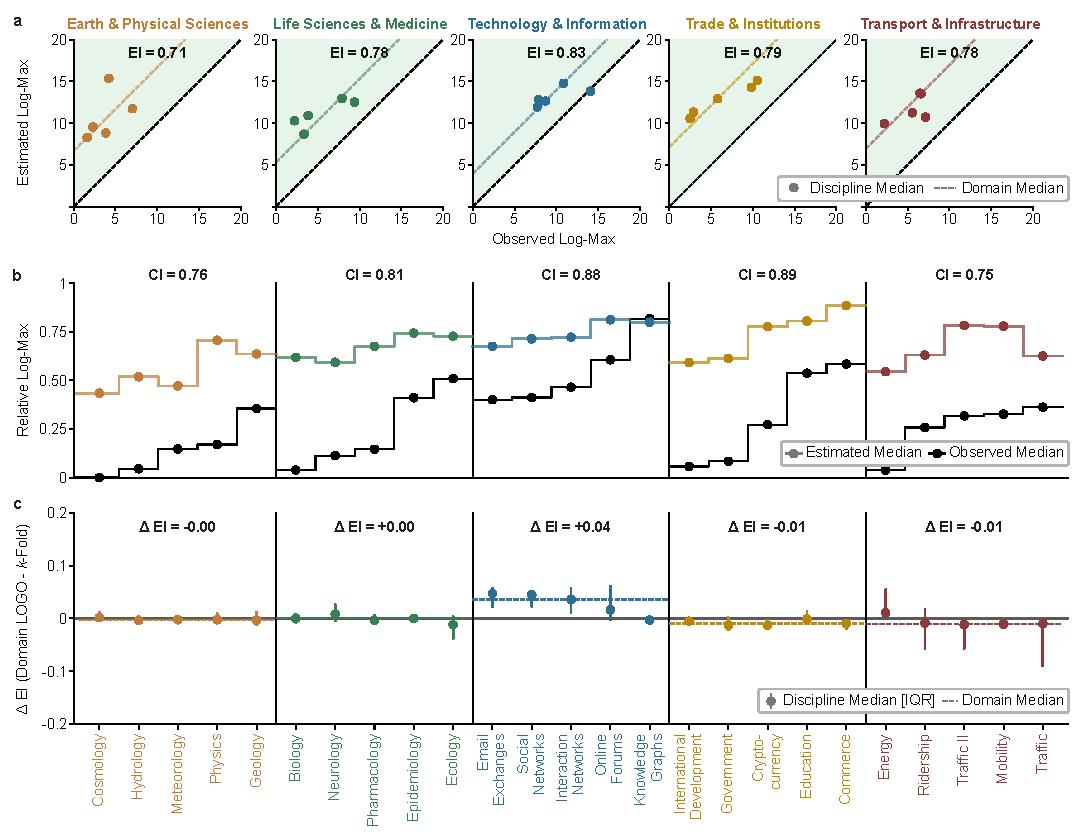
\includegraphics[width=\linewidth]{fig2.pdf}
\caption{
    \textbf{Domain transfer of the capacity frontier.} Domain-level LOGO-CV across 25 disciplines in 5 broad domains. \textbf{a}. Estimated versus observed log-maxima for each withheld domain (top columns). Discipline medians (domain-colored markers) fall along domain offsets (domain-colored dashed lines) relative to equality (gray dashed diagonal). Green shading marks conservative estimates at or above observed maxima. \textbf{b}. Estimation-observation consensus profiles within withheld domains (middle row). Step traces and markers show observed log-maxima (black trace on bottom) and median model estimates (domain-colored trace on top), with disciplines ordered by observed maximum and profiles scaled to the unit interval. \textbf{c}. Paired differences in frontier efficiency between random cross-validation ($5$-Fold-CV and $10$-Fold-CV) and domain-level LOGO-CV ($\text{random} - \mathrm{LOGO}$, bottom row). Markers and vertical intervals show discipline medians and interquartile ranges across models (domain-colored intervals), dashed lines show domain medians (domain-colored dashed lines), and the horizontal band spans the interquartile range of baseline variation from model means (light blue band). Annotations report domain EI (\textbf{a}), domain CI (\textbf{b}), and domain-median $\Delta\mathrm{EI}$ (\textbf{c}).
}
\label{fig:transfer}
\end{figure}

\subsection*{Consensus Across Paradigms}
\label{sub-sec:consensus}
The capacity frontier was consistent across learning paradigms (Fig.~\ref{fig:consensus}). 9 independent estimators across 3 distinct learning paradigms agreed on their predicted frontier values. The learning paradigms were linear parametric, non-linear ensemble, and neural networks. All 9 models were trained on the same vectors $x'$ and $z'$ while the estimators differed in functional form, regularization, and optimization. Each test was repeated 30 times to reduce sensitivity to parameter initialization and optimization stochasticity. Predicted frontier values were averaged across repetitions. Pairwise model consensus across all 36 pairs of seed-averaged predictions was 0.84. A geometric mean this close to 1 simultaneously required high rank agreement, top-weighted overlap, and statistical dependence, such that no single component could carry the outcome. Spearman rank correlation, rank-biased overlap, and distance correlation were 0.82, 0.85, and 0.80, respectively. The agreement was evaluated on in-sample analyses using full-corpus fits. Consensus across the tested learning paradigms indicated that the frontier reflected a regularity, which was unlikely an artifact of inductive bias.

%% stress tests
\subsection*{Stable Under Perturbation}
\label{sub-sec:perturb}
The capacity frontier was robust to perturbation (Fig.~\ref{fig:tests}a, Fig.~\ref{fig:tests}b, Supplementary Table~\ref{tab:si-perturb}). The 12 perturbations targeted 4 categories: network substrates, graph invariants, dynamical processes, and process signatures. Under domain-level LOGO-CV, the frontier was trained on the original data, the model frozen, then evaluated on the perturbed data in the withheld domain. Each test was repeated 30 times and averaged across repetitions to reduce sensitivity to perturbation realization and estimator initialization. Paired differences were computed by subtracting the original outcomes from the perturbed ones across 45 estimator-by-domain comparisons, where negative values indicated lower performance. At the highest tested intensity, median paired differences in frontier efficiency ranged from -0.02 to +0.01. Median paired differences in estimation-observation consensus were 0.00 for all network and invariant perturbations. Median paired differences in consensus were -0.04 for process bootstrapping, -0.02 for process scaling, and -0.06 for process smoothing. Signature jitter, noise, and masking produced median consensus differences of -0.01, -0.03, and -0.06, respectively. Paired Wilcoxon Two One-Sided Tests (TOST) across 45 estimator-by-domain comparisons supported equivalence for all 12 perturbations within their empirically derived margins ($\delta_{\mathrm{EI}} = 0.09$ and $\delta_{\mathrm{CI}} = 0.15$, all Holm-adjusted $p < 0.001$). Response curves across normalized perturbation intensity were descriptive, where only the highest perturbation intensity was formally tested. Nevertheless, the frontier could withstand bounded structural alterations, process distortions, and feature noise while remaining reliable.

\subsection*{Degradation Under Falsification}
\label{sub-sec:falsify}
The capacity frontier predictably degraded under falsification (Fig.~\ref{fig:tests}c, Supplementary Table~\ref{tab:si-falsify}). There were 3 falsification procedures that disrupted the correspondence between feature representations and target maxima in distinct ways: target permutation preserved the empirical target distribution, random generation sampled within observed feature ranges, and vector generation maintained approximate featurewise scale. Under domain-level LOGO-CV, the frontier was evaluated by freezing the models after training on the original data, and separately after retraining on the falsified data. Each test was repeated 30 times and averaged across repetitions to reduce sensitivity to estimator initialization and training stochasticity. Paired differences were computed by subtracting the original outcomes from the falsified ones across 45 estimator-by-domain comparisons, where negative values indicated lower performance. Under the frozen model, median paired differences in frontier efficiency were -0.02 for target permutation, -0.05 for random generation, and -0.03 for vector generation. After retraining, median paired differences in frontier efficiency were -0.08 for target permutation, -0.03 for random generation, and -0.03 for vector generation. Median paired differences in estimation-observation consensus were -0.24, -0.24, and -0.21 when frozen, and -0.33, -0.21, and -0.28 after retraining, respectively. Paired One-Sided Wilcoxon Signed-Rank Tests supported lower efficiency and lower consensus across all 12 comparisons (all Holm-adjusted $p \le 0.005$ for efficiency and $p < 0.001$ for consensus). The falsified corpora served as prespecified negative controls. They indicated that the frontier depended on a true representation–target correspondence.

\subsection*{Parsimony Under Ablation}
\label{sub-sec:ablate}
No alternative capacity frontier specification meaningfully outperformed the log-additive decomposition (Fig.~\ref{fig:tests}d, Supplementary Table~\ref{tab:si-ablation}). The 4 alternative specifications contained simple ablations: invariants only and signatures only, and complex ablations: joint features and interaction terms. Invariants only trained the frontier using $x'$ alone, while  signatures only used $z'$. Joint features combined both vectors into a single-stage fit, while interaction terms augmented the log-additive decomposition with pairwise products between the 2 vectors. Under domain-level LOGO-CV, ablations were fit on each training set and evaluated on the corresponding test set. Each test was repeated 30 times and averaged across repetitions to reduce sensitivity to estimator initialization and training stochasticity. Paired differences were computed by subtracting outcomes from the original formulation from the ablated ones across 45 estimator-by-domain comparisons, where negative values indicated lower performance. Median paired differences in frontier efficiency were -0.01 for invariants only, joint features, and interaction terms, and 0.00 for signatures only. Median paired differences in estimation-observation consensus were -0.30 for invariants only, -0.09 for signatures only, -0.26 for joint features, and -0.08 for interaction terms, respectively. Paired One-Sided Wilcoxon Signed-Rank tests supported non-inferiority of the log-additive decomposition to all 4 alternatives in both metrics within their empirically derived margins ($\delta_{\mathrm{EI}} = 0.07$ and $\delta_{\mathrm{CI}} = 0.14$, all Holm-adjusted $p < 0.001$). These tests limited alternative advantages. They supported the log-additive decomposition as the parsimonious formulation of the frontier.

%% fig 3
\begin{figure}[H]
\centering
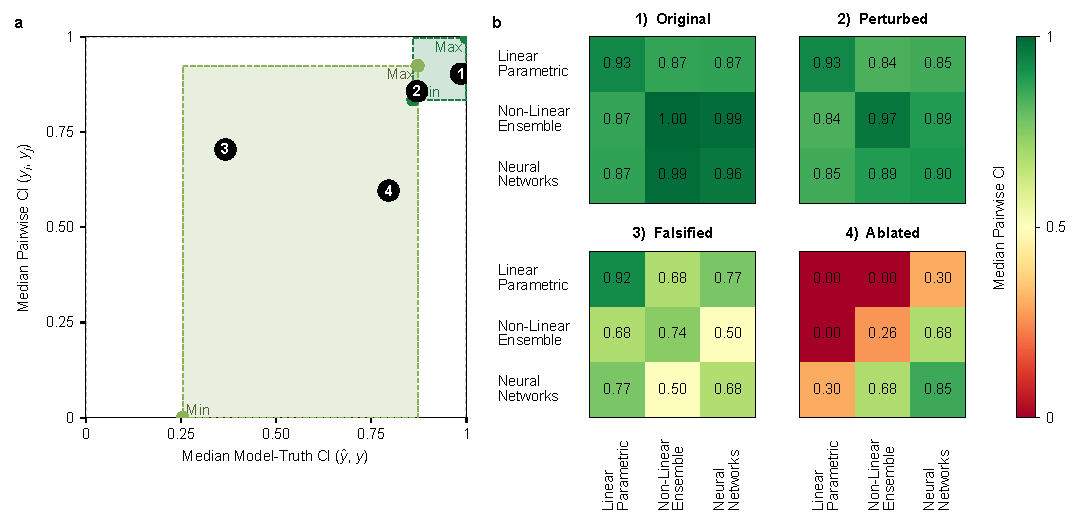
\includegraphics[width=\linewidth]{fig3.pdf}
\caption{
    \textbf{Learning paradigm and estimation-observation consensus.} Agreement across 9 estimators in 3 learning paradigms evaluated on full-corpus fits across 30 seeds. \textbf{a}. Median estimation-observation consensus ($\widehat{y}^*$ versus $y^*$) by median pairwise model consensus ($\widehat{y}^*_i$ versus $\widehat{y}^*_j$). Points mark the tests: (1) original, (2) perturbed, (3) falsified, and (4) ablated. Shaded rectangles span coordinate-wise ranges of paradigm medians for the original and perturbed (green) and falsified and ablated (yellow) groups. \textbf{b}. Median pairwise model consensus across learning paradigms for each test in \textbf{a} with paradigm agreement along the diagonal axes.
}
\label{fig:consensus}
\end{figure}

\begin{figure}[H]
\centering
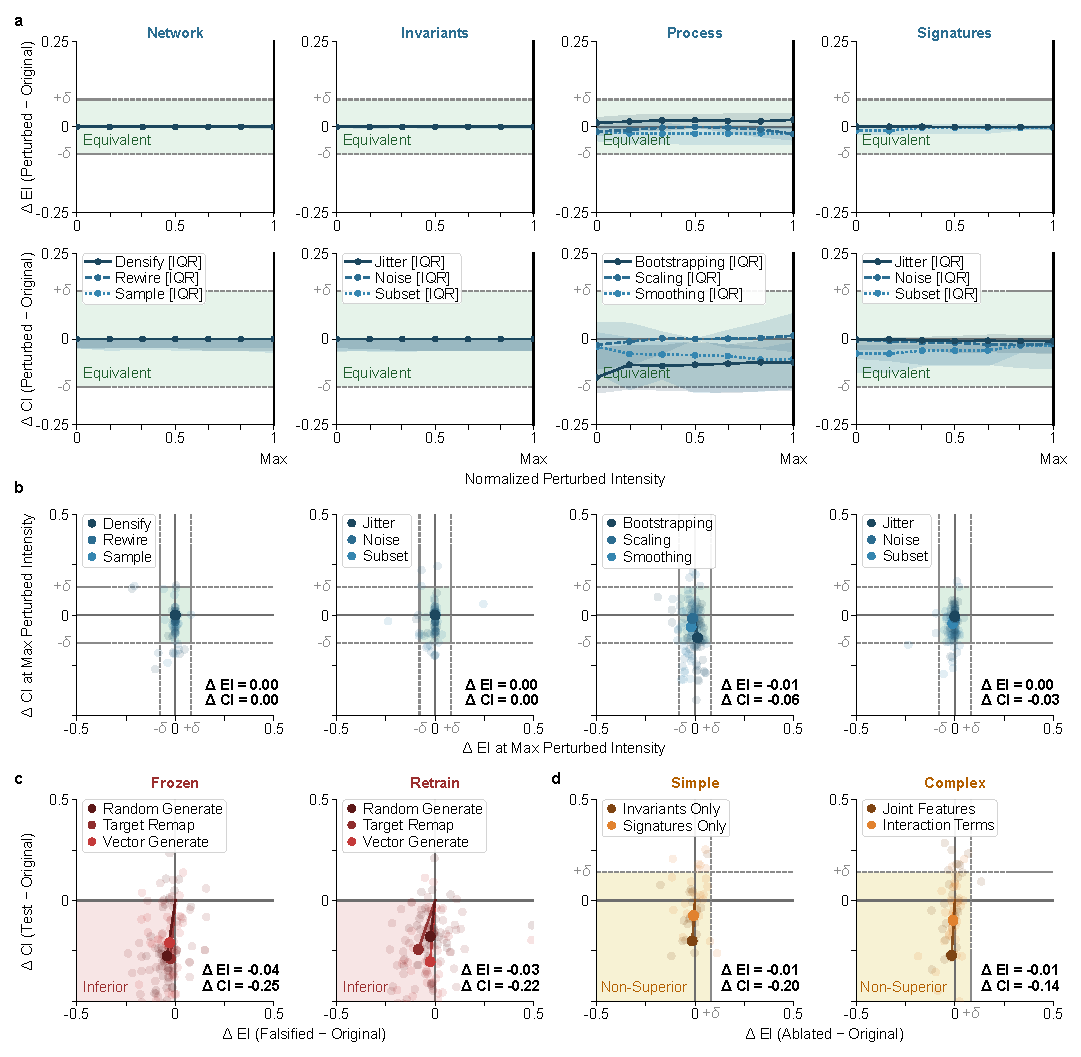
\includegraphics[width=\linewidth]{fig4.pdf}
\caption{
    \textbf{Stress tests of the capacity frontier.} Paired shifts across 45 estimator-by-domain comparisons under domain-level LOGO-CV, computed as tested condition minus original condition, or alternative specification minus log-additive decomposition. \textbf{a}. Response curves across normalized intensity for 12 perturbations in 4 categories, with $\Delta\mathrm{EI}$ above and $\Delta\mathrm{CI}$ below. Lines and shaded bands show medians and interquartile ranges. \textbf{b}. Paired shifts at maximum perturbation intensity. \textbf{c}. Falsification shifts under frozen and retrained frontiers for target permutation, random generation, and vector generation. The red quadrant marks joint degradation ($\Delta\mathrm{EI} < 0$, $\Delta\mathrm{CI} < 0$). \textbf{d}. Simple (invariants only, signatures only) and complex (joint features, interaction terms) specifications compared with the log-additive decomposition. In \textbf{b--d}, faint points show individual comparisons and solid points show coordinate-wise medians connected to the origin. Green regions (\textbf{a}, \textbf{b}) mark perturbation equivalence margins ($\delta_{\mathrm{EI}} = 0.09$, $\delta_{\mathrm{CI}} = 0.15$), and the yellow region (\textbf{d}) marks the ablation non-inferiority margin ($\delta_{\mathrm{EI}} = 0.07$, $\delta_{\mathrm{CI}} = 0.14$).
}
\label{fig:tests}
\end{figure}

%% discussion
\section*{Discussion}
The capacity frontier makes empirical maxima comparable across disciplinary boundaries. A frontier with either a broad domain or individual discipline withheld from training bounded empirical maxima with performance comparable to random resampling. Information from one system was therefore useful for estimating the maxima in another despite differences in subject, size, scale, units, and dynamics. These comparisons provide a basis for asking which constraints are shared across systems and which depend on domain specificity. Capacity estimation can therefore use empirical evidence beyond a system’s own substantive boundary.

The capacity frontier does not require a model of the dynamical processes. Graph invariants and process signatures support capacity estimation without training domain specific models or simulating their dynamics. Domain specific models are still important for causal explanation and intervention, but SCT provides a standard benchmark as a complement. Interpreting this benchmark requires additional inquiry, as the reported slack above the maxima was nearly three orders of magnitude. This gap may reflect a loose statistical envelope, unequal observation windows, or differences in measurement conventions. Although the meaning of the slack remains open, the capacity frontier still placed most evaluated maxima below its estimates without a traditional model of the underlying dynamics.

Selective stability demonstrates why the capacity frontier is informative. Perturbations at the highest tested intensity preserved the frontier's original performance. Falsifications that deliberately destroyed the representation–target correspondence degraded frontier performance, which was unrecoverable even after retraining. Consensus among learning paradigms was relatively high and comparatively similar between the original and perturbed conditions. Only after falsification and ablation did the model consensus between learning paradigms degrade. This supports the frontier as a non-spurious object, distinguishable from a flexible upper envelope.

The capacity frontier is jointly determined and decomposable. Removing either component or combining them without log-additivity did not improve frontier performance or consensus among estimators. The results support the log-additive decomposition, but leave its exhaustiveness unresolved. All findings were conditioned on the 5 broad domains, 21 graph invariants, 7 process signatures, 3 learning paradigms, the log-additive decomposition, and the prespecified daily aggregation. Broader corpora, different vector representations, more diverse learning paradigms, and alternative temporal scales all provide direct tests of SCT.

%% methods
\section*{Methods}
\subsection*{N3S Definition}
Within SCT, an N3S was defined by 3 components. The 1st was a network substrate: a finite set of elements with a relational or attribution structure expressible as a fixed graph $G$. The 2nd was a dynamical process, a time-indexed sequence of discrete events observed directly or reconstructed from published canonical timings, with each event admitting a substantively defined correspondence to substrate elements. The 3rd was a measurement convention, a source-native or prespecified operational rule that converted the sequence into a rate from which an empirical maximum could be computed. A system qualified as an N3S when its source records supported all 3 components. Operational recastings were fixed before analysis and documented in Supplementary Table~\ref{tab:si-corpus}, so membership fixed the scope of SCT before any test of it. Systems lacking an identifiable substrate, or supplying only aggregate quantities without a definable correspondence, fell outside the class and were not evaluated.

\subsection*{Data and Corpus Composition}
The corpus contained 25 data sets spanning 5 broad domains, each contributing 5 individual disciplines: Earth \& Physical Sciences, Life Sciences \& Medicine, Technology \& Information, Trade \& Institutions, and Transportation \& Infrastructure. All datasets were derived from publicly available records, with sources, access details, operational recastings, and per-system definitions reported in Supplementary Table~\ref{tab:si-corpus}. Observation windows were the system-specific source periods or canonical intervals and were not standardized in duration. Network substrates spanned 5 to roughly 10,400,000 nodes and 10 to roughly 7,200,000,000 edges, and empirical maxima spanned 3 to roughly 1,300,000 observations per day. Measurements did not share any units before encoding, and daily aggregation was the common temporal convention. Each system contributed exactly 1 analysis record consisting of its graph invariants, its process signatures, and its empirical maximum.

\subsection*{Network Substrate Construction}
Each network substrate was represented as a finite, simple, undirected graph with node set $V$ and edge set $E$ comprising unordered node pairs,

\begin{equation}
G \;=\; (V, E),
\qquad
E \subseteq \binom{V}{2}
\end{equation}

where nodes represented the units to which observations were attributed and edges represented either the system's source relation or a prespecified operational relation among those units. Each observation $o$ in the observation set $\mathcal{O}$ admitted this correspondence, expressible as an attribution map $a: \mathcal{O} \rightarrow V \cup E$ linking the dynamical process to its substrate, where measured correspondences were not required. Directed or weighted records were converted to undirected, unweighted edges, and the substrate was held fixed over each system's observation window. Interaction records were represented by the union of observed pairs or by a complete bipartite recasting over documented entity classes, including entity-time constructions. Multi-edges and self-loops were removed, and isolated vertices were retained. Complete bipartite substrates (college, email, mooc, overflow) were represented by their partition sizes and evaluated using closed-form expressions for $K_{m,n}$ under the definitions of Supplementary Table~\ref{tab:si-features}. Node and edge definitions for every system are given in Supplementary Table~\ref{tab:si-corpus}.

\subsection*{Dynamical Process Construction}
Each dynamical process was represented from source records without generating synthetic observations. Most systems supplied an observed event stream. Where only population-mean transition times were available, they were recast as a canonical event sequence rather than as individual-level observations. Events were linked to the substrate through the attribution map. Where source records were continuous measurements, observations were defined by the prespecified operational discretization reported for that system in Supplementary Table~\ref{tab:si-corpus}. Event counts were aggregated to calendar days, in UTC where records carried a time of day, or to consecutive 24-hour bins from the first record where sources supplied relative times or snapshot sequences, giving a single rate series,
\begin{equation}
S \;=\; \left\{ r_{t} \right\}_{t \in T},
\qquad
r_{t} \;=\; \frac{n_{t}}{\Delta t},
\qquad
\Delta t \;=\; 1\ \mathrm{day}\ (24\ \mathrm{hours})
\label{eq:series}
\end{equation}
where $n_{t}$ is the observation count in interval $t$ and $T$ is the chronologically ordered set of intervals in the series. For 19 systems, $T$ comprised the days with at least 1 recorded event, so days without events were omitted. Metrla, pemsbay, montevideo, windmill, and wiki supplied regular snapshots that aggregate to complete daily series. Chickenpox supplied weekly county totals, each converted to its daily average and entered as 1 series value at its report date. Crop records were resolved to the sampling month, so each monthly total entered as 1 series value on the 1st day of its month. Supplementary Table~\ref{tab:si-corpus} lists the convention for each system. This series served two roles. Its temporal shape defined the process signatures, so the 7 signature summaries were computed from the same trajectory whose maximum defined the estimation target. Held-out evaluation therefore predicts the maxima of held-out systems without observing those maxima or using the raw held-out trajectories as model inputs, though the trajectory summaries were derived from the same series. The Fano factor retains the count scale of the series, so its ratio to the squared coefficient of variation equals the series mean $\bar{r}$. The remaining 6 signatures are scale-free. No fitted dynamical model or generative mechanism entered the construction.

\subsection*{Empirical Maximum Target}
For each system, the maximum rate observed in its finite series $S$ at $\Delta t = 1$ day was $r_{\max} = \max_{t \in T} r_t$, where $T$ is the interval set of Eq.~\eqref{eq:series}. A sample maximum can be more extreme over longer observation windows \citep{ref58,ref59,ref60}. Windows differed across systems and no common horizon was imposed, so all targets and frontiers are conditional on the windows in Supplementary Table~\ref{tab:si-corpus}. The estimation target, 1 value per system, was the log-transformed maximum
\begin{equation}
y^{*} \;=\; \ln\!\left(1 + r_{\max}\right)
\label{eq:maximum}
\end{equation}
The logarithm places maxima spanning more than 5 orders of magnitude on a common scale, and the unit shift accommodates 0 counts. Slack and violation magnitudes are therefore in natural-log units, while VR, normalized MV and MS, EI, and CI are dimensionless. $F(x', z')$ was fitted as a statistical upper envelope of these finite-window maxima in the shared representation. Its empirical violations were measured directly by VR and MV, with no claim of a bound over all dynamics on $G$.
\subsection*{Encoding and Standardization}
The graph-invariant vector collected 21 classical whole-graph quantities spanning 5 families: cardinality and cut structure, cohesion, an extremal statistic, degree-distribution statistics, and spectral moments,
\begin{equation}
x \;=\; \phi(G) \;=\; (x_1, x_2, \ldots, x_{21}) \;\in\; \mathbb{R}^{21}.
\end{equation}
The process-signature vector collected 7 summaries of the series $S$ in chronological order, covering temporal dependence, dispersion, local volatility, long-range dependence, trend, and distributional asymmetry,
\begin{equation}
z \;=\; \psi(S) \;=\; (z_1, z_2, \ldots, z_7) \;\in\; \mathbb{R}^{7}.
\end{equation}
Admission followed prespecified criteria: every quantity had to be classical, global to the graph or series, defined without external parameters or arbitrary thresholds, exactly and deterministically computable at the largest corpus scales, and finite on all corpus systems. Full definitions, citations, and computational notes are reported in Supplementary Tables~\ref{tab:si-features} and \ref{tab:si-signatures}. Standardization mapped each coordinate to 0 mean and unit variance with the population standard deviation,
\begin{equation}
x' \;=\; \frac{x - \mu_x}{\sigma_x},
\qquad
z' \;=\; \frac{z - \mu_z}{\sigma_z},
\end{equation}
with the data on which this mapping was fitted governed by the resampling protocol below.
\subsection*{Capacity Frontier Learning}
The 28 predictors outnumber the 25 systems, so an unconstrained learner could interpolate the corpus. Complexity was therefore constrained by a stagewise form whose stages see at most 21 or 7 coordinates and by fixed, prespecified estimator settings without estimator-specific tuning. Repetition over 30 seeds assessed Monte Carlo stability, and 9 estimators from 3 learning paradigms assessed sensitivity to inductive bias.
The fitted frontier took the log-additive stagewise form \citep{ref67} with an identifiability constraint on the process stage,
\begin{equation}
\widehat{y}^* = F(x', z') = f_C(x'; \tau_C) + f_R(z'; \tau_R)
\label{eq:frontier}
\end{equation}
Stage 1 fitted $f_C$ to $y^{*}$ by asymmetric regression at $\tau_C = 0.99$, placing the fit near the upper envelope of the maxima given the graph invariants \citep{ref29}. Stage 2 fitted $f_R$ to the signed slack $y^{*} - \hat{f}_C(x')$ at $\tau_R = 0.50$, modeling how the dynamical process modulates the structural bound. The identifiability constraint subtracted the training mean of $f_R$, assigning overall level to $f_C$ and modulation to $f_R$, and the prediction summed the 2 stages. $\tau_C$ sets the asymmetry of the structural stage and does not fix the nominal coverage of the sum, so envelope behavior was evaluated empirically by VR, MV, MS, and EI.
9 estimators instantiated this form with the same asymmetry levels, the same 2-stage protocol, and fixed hyperparameters, with library defaults for any setting not stated here. The linear parametric paradigm comprised linear quantile regression \citep{ref22} minimizing the mean pinball loss plus $\alpha \lVert \beta \rVert_1$ with $\alpha = 0.1$ (HiGHS solver), linear asymmetric weighted least squares \citep{ref36} minimizing $(2n)^{-1} \sum_{i=1}^{n} w_i e_i^{2} + \alpha \lVert \beta \rVert_1$ over the $n$ training systems, where $e_i$ is the residual, $\alpha = 0.1$, and the expectile weight $w_i$ is $\tau$ for $e_i \ge 0$ and $1 - \tau$ otherwise, and a concave-envelope regressor that fits a linear quantile score ($\alpha = 0.1$) and linearly interpolates the concave upper envelope of the maxima at each score, held constant beyond its end points. The weighted least squares initialized coefficients to zero, setting the stage-1 intercept to the training target mean, and alternated expectile weight updates with cyclic coordinate descent \citep{ref76} until the largest coefficient change fell below $10^{-4}$ or 1,000 passes elapsed, with an unpenalized intercept in stage 1 and no intercept in stage 2. The non-linear ensemble paradigm comprised a quantile random forest \citep{ref37} (100 fully grown trees), gradient-boosted quantile regression \citep{ref38} (100 trees, maximum depth 3, learning rate 0.1), and XGBoost under its quantile objective \citep{ref39} (100 trees, maximum depth 6, learning rate 0.3, $\ell_2$ penalty $\lambda = 1$). The neural network paradigm comprised multilayer perceptrons trained with pinball loss and with expectile loss, and an input-convex network \citep{ref40} trained with pinball loss whose weights beyond the input layer were made non-negative by absolute value. All 3 used hidden layers of 8 and 4 units with ReLU activations \citep{ref80} and dropout 0.1 \citep{ref77}, an output bias initialized to the stage-level quantile of the training targets, and full-batch AdamW \citep{ref41} (learning rate 0.1, weight decay 0.01, 1,000 epochs, gradient-norm clipping at 5.0), with predictions clipped to the training-target range.
\subsection*{Performance Metrics}
Frontier quality was summarized by the Efficiency Index (EI) \citep{ref103,ref111}. For targets $y^{*}$ and frontier values $\hat{y}$, the violation rate VR is the fraction of systems with $y^{*} > \hat{y}$, the mean violation MV is the mean exceedance among violators (0 when none occurred), and the mean slack MS is the mean of $\max(\hat{y} - y^{*}, 0)$ over all evaluated systems. EI is the geometric mean of 3 bounded scores, with MV and MS normalized by the mean absolute target $\overline{\lvert y^{*} \rvert} = n^{-1}\sum_{i=1}^{n} \lvert y_i^{*} \rvert$ of the evaluated sample:
\begin{equation}
\mathrm{EI} \;=\;
\Big[
(1 - \mathrm{VR})
\Big(1 + \frac{\mathrm{MV}}{\overline{\lvert y^{*} \rvert}}\Big)^{-1}
\Big(1 + \frac{\mathrm{MS}}{\overline{\lvert y^{*} \rvert}}\Big)^{-1}
\Big]^{1/3} \in [0, 1].
\end{equation}
EI reaches 1 only when the frontier is never violated and carries no slack, and $1 - \mathrm{VR}$ was floored at $10^{-12}$ for numerical stability.
Agreement between 2 vectors was summarized by the Consensus Index (CI), the geometric mean of Spearman rank correlation \citep{ref42} rescaled to $\rho_s^{+} = (1 + \rho_s)/2$, top-weighted rank-biased overlap (RBO) \citep{ref43}, and distance correlation ($\mathrm{dCor}$) \citep{ref44},
\begin{equation}
\mathrm{CI} \;=\;
\Big[
\rho_s^{+}\ \mathrm{RBO}\ \mathrm{dCor}
\Big]^{1/3} \in [0, 1].
\end{equation}
RBO used persistence $p = 0.9$ on descending rankings with ties ordered by index, extrapolating the unobserved tail from the agreement at the final depth, and dCor used the standard (V-statistic) sample estimator. Components were clipped to $[0, 1]$ to correct floating-point error, Spearman correlation was set to 0 when either vector was constant, and CI required at least 2 systems. CI is a descriptive measure without calibration against a chance-level null, and a high CI indicates simultaneous global rank agreement, agreement among the top-ranked systems, and statistical dependence. CI served 2 roles: estimation-observation consensus between predicted frontier values and observed maxima, and pairwise model consensus between the seed-averaged predictions of estimator pairs.
\subsection*{Resampling and Leakage Control}
Under a single leakage rule, all data-dependent mappings, comprising the standardizers of $x$ and $z$, every estimator stage, and the training mean subtracted from $f_R$ in Eq.~\eqref{eq:frontier}, were fitted on the training rows of the active split only, with estimators cloned per fold. All encoded quantities were finite, so no rows were excluded, and the log target transform has no fitted parameters. 4 resampling regimes applied this rule: repeated random $5$-Fold-CV and $10$-Fold-CV over 30 repetitions with partitions drawn by scikit-learn \texttt{RepeatedKFold} under random state 42 \citep{ref73}, and leave-one-group-out cross-validation (LOGO-CV) \citep{ref74} withholding 1 broad domain (5 folds) or 1 system (25 folds) to evaluate generalization across structured environments \citep{ref68,ref69,ref70,ref107}. LOGO partitions are deterministic, so their 30 repetitions varied model-fitting seeds only. In every regime, repetition $b = 0, \ldots, 29$ used model-fitting seed $42 + b$. Frontier metrics were computed within each test fold for each seed and averaged over folds and repetitions. CI was computed within each withheld domain from out-of-fold predictions averaged over the 30 seeds. Under system-level LOGO-CV, where a single-system fold leaves correlation undefined, out-of-fold predictions were pooled within each domain before computing CI. For resampling equivalence, the averaged out-of-fold predictions of each regime were rescored within each of the 5 domains, giving 1 EI and 1 estimation-observation CI per estimator, domain, and regime.

Stress tests used 2 tracks. The frozen track applied models and standardizers fitted on unmodified training data to modified held-out data. The retrained track refitted the full pipeline on modified data under the same protocol. The leakage rule had 2 exceptions, both constructed across all systems before splitting: the falsified corpora, including target permutations and the ranges and pools used to generate synthetic features, and the corpus-wide sample standard deviations of the raw coordinates that scale additive feature noise. Models and standardizers remained training-fold specific, and falsification was treated as a corpus-level negative control.

\subsection*{Evaluation and Reporting Conventions}
Each Results section mapped to 1 protocol. Shared-coordinate frontier quality used repeated $5$-Fold-CV and $10$-Fold-CV, and domain transfer used LOGO-CV at domain and system level. Cross-paradigm consensus was descriptive and in-sample: all 9 estimators were trained on the full corpus over 30 seeds, and the 36 pairs of seed-averaged predictions were compared by CI. The comparisons of Fig.~\ref{fig:consensus} used descriptive full-corpus predictions rather than the 45-cell inference panel described below. The original condition fitted all 9 estimators on the full corpus over 30 seeds. The perturbed condition applied the frozen full-corpus fits to each intervention at its most severe intensity on all 25 systems, with realization $b$ of a stochastic intervention scored by the fit of seed $42 + b$ and predictions averaged over realizations. The falsified condition scored the frozen full-corpus fits on each falsified corpus. The ablated condition refitted each specification on the full corpus over 30 seeds. Each value was the median CI over model pairs. Perturbation (frozen track), falsification (both tracks), and ablation (retrained track) used domain-level LOGO-CV. Benchmarks were domain-level LOGO-CV for resampling equivalence, the original condition for perturbation and falsification, and the log-additive decomposition for ablation.

Inference used the fixed, prespecified panel $\mathcal{P}$ of 45 estimator-by-domain cells (9 estimators by 5 withheld domains), each averaged over 30 seeds before testing. For metric $M$, estimator $m$, and withheld domain $d$, the paired difference was $d_{md} = M^{\mathrm{comparison}}_{md} - M^{\mathrm{benchmark}}_{md}$, and the estimand was the panel median $\theta_{\mathcal{P}} = \operatorname{median}_{(m,d) \in \mathcal{P}} d_{md}$. The 45 cells share estimators, training systems, and withheld domains, so their outcomes may co-vary and inference is conditional on this panel. Its $p$ values indicate a consistent shift across the panel and may be optimistic under strong within-domain or within-estimator correlation. All tests were one-sided Wilcoxon signed-rank tests \citep{ref45}, computed by \texttt{scipy.stats.wilcoxon} under default settings that discard zero differences, with Holm-Bonferroni adjustment \citep{ref46} within each test family and a significance threshold of 0.05 after adjustment. Effect sizes were rank-biserial correlations $(W_{+} - W_{-})/(W_{+} + W_{-})$ computed from the nonzero, unshifted differences, where $W_{+}$ and $W_{-}$ are the positive and negative rank sums \citep{ref71}. Equivalence for resampling and perturbation used 2 one-sided tests (TOST) \citep{ref47}:
\begin{equation}
H_{01}:\; \theta \le -\delta,
\qquad
H_{02}:\; \theta \ge \delta.
\end{equation}
Each null was tested one-sidedly on the paired differences shifted by $-\delta$ or $+\delta$, equivalence was concluded when both were rejected, and the TOST $p$ value was the larger of the 2. Each margin $\delta$ was the interquartile range of the benchmark values, floored to the 2nd decimal and computed separately for EI and CI. Benchmark values were the 9 model-level domain LOGO-CV means, each averaged equally across the 5 domains, for resampling equivalence ($\delta_{\mathrm{EI}} = 0.01$, $\delta_{\mathrm{CI}} = 0.03$), the 45 panel values under the original condition for perturbation ($\delta_{\mathrm{EI}} = 0.09$, $\delta_{\mathrm{CI}} = 0.15$), and the 45 panel values under the log-additive decomposition for ablation ($\delta_{\mathrm{EI}} = 0.07$, $\delta_{\mathrm{CI}} = 0.14$). The margins express tolerance relative to benchmark variability, and treating them as substantively negligible would require independent justification. Where intervention intensity varied, response curves were reported descriptively. Only the most severe intensity was formally tested. Severity was the intensity value for rewiring, densification, node removal, noise, jitter, and smoothing, 1 minus the retention for masking, 1 minus the support for bootstrap resampling, and $\lvert \ln \gamma \rvert$ for power scaling (Supplementary Table~\ref{tab:si-protocol}).

\subsection*{Perturbation, Falsification, Ablation}
Perturbation tested stability under 12 interventions, 3 in each of 4 categories (network substrates, graph invariants, dynamical processes, and process signatures), each applied per system at 7 graded intensities (Supplementary Table~\ref{tab:si-protocol}). Network interventions at intensity $s$ were degree-preserving rewiring \citep{ref56} with $\max(1, \lfloor s\lvert E \rvert \rfloor)$ rewiring trials that never create multi-edges or self-loops, random edge densification \citep{ref106} adding $\lfloor s\lvert E \rvert \rfloor$ edges drawn uniformly without replacement from non-adjacent vertex pairs, and uniform node removal \citep{ref104,ref105} deleting $\lfloor s\lvert V \rvert \rfloor$ vertices drawn without replacement, after which invariants were recomputed. The 4 complete bipartite substrates received exact node removal and deterministic closed-form approximations for rewiring and densification (\hyperref[sec:si-note-bipartite]{Supplementary Note 1}). Invariant and signature interventions acted on the raw vector $x$ or $z$ before standardization. Additive noise added $\mathcal{N}(0, (s\sigma_j)^2)$ to coordinate $j$, where $\sigma_j$ is its sample standard deviation across the 25 systems. Multiplicative jitter multiplied coordinate $j$ by $1 + \varepsilon_j$ with $\varepsilon_j \sim \mathcal{N}(0, s^2)$ and clipped originally non-negative coordinates at 0. Masking at retention $\rho$ kept $\lfloor \rho p \rfloor$ of the $p$ coordinates, chosen uniformly, and set the others to 0. Process interventions acted on the series of Eq.~\eqref{eq:series} through power scaling $r_t' = (r_t + 1)^{\gamma} - 1$, trailing rolling means over $w$ consecutive values with fewer values averaged at the start of the series, or bootstrap resampling \citep{ref75} at support $s$, which drew $k = \max(1, \operatorname{round}(s\lvert T \rvert))$ values with replacement and filled the remaining $\lvert T \rvert - k$ positions by resampling those $k$ values, destroying temporal order. Signatures were recomputed from the modified series, and targets remained the observed maxima.

Falsification tested degradation under 3 procedures that destroyed the correspondence between representation and maxima (Supplementary Table~\ref{tab:si-protocol}). Target permutation assigned each system the complete event record, and hence the $y^{*}$, of another system through a cross-domain derangement, leaving $x$ and $z$ unchanged and preserving the target distribution. Random generation redrew every raw coordinate independently from a uniform distribution over its range across the 25 systems, preserving feature support. Vector generation drew every raw coordinate from its 25 corpus values with replacement and added Gaussian noise with standard deviation equal to that coordinate's population standard deviation across the corpus, preserving approximate featurewise scale. Falsified corpora were generated once under base seed 42. Each procedure and track tested $H_0: \theta \ge 0$ against $H_1: \theta < 0$ with Holm adjustment across the 6 procedure-by-track comparisons for each metric, and degradation was concluded when the adjusted $p$ value was below 0.05 and the median difference was negative.

Ablation tested representation dependence under 4 input specifications, each refitted with the prespecified estimator settings. The simple specifications fitted the stage-1 estimator at $\tau_C = 0.99$ in a single stage on invariants only ($x'$) or signatures only ($z'$). The complex specifications were joint features, a single stage at $\tau_C = 0.99$ on concatenated $x'$ and $z'$, and interaction terms, the log-additive decomposition with the 147 products $x_j z_k$ of raw coordinates appended to the process stage so that $f_R$ received 154 inputs standardized within each fold. With $d_{md}$ taken as the alternative minus the log-additive decomposition, non-inferiority of the log-additive decomposition tested $H_0: \theta \ge \delta$ against $H_1: \theta < \delta$ on EI and CI by one-sided Wilcoxon signed-rank tests \citep{ref78} applied to $d_{md} - \delta$. Holm adjustment was applied separately to the 2 complex and the 2 simple specifications for each metric, and non-inferiority was concluded when the adjusted $p$ value was below 0.05 and the median difference was below $\delta$.

\subsection*{Implementation and Reproducibility}
All analyses were implemented in Python 3.11 \citep{ref86,ref102}. Graph construction and invariants used python-igraph 1.0.0 \citep{ref48,ref93} with NumPy 2.3.5 \citep{ref81,ref96}, SciPy 1.16.3 \citep{ref82,ref97}, and pandas 3.0.0 \citep{ref83,ref84}. Network construction for the street substrate used networkx 3.5 \citep{ref91,ref98} and OSMnx 2.0.6 (Supplementary Reference~\ref{src:S22}), and the benchmark temporal-graph datasets were loaded through torch-geometric 2.7.0 \citep{ref89,ref99} and torch\_geometric\_temporal 0.56.2 \citep{ref90,ref100}. GWOSC and Meteostat records were retrieved with gwosc 0.8.1 and meteostat 1.7.6. Estimators used scikit-learn 1.8.0 \citep{ref72,ref94}, sklearn-quantile 0.1.1 \citep{ref87}, XGBoost 3.1.1 \citep{ref39,ref95}, and PyTorch 2.9.0 \citep{ref85,ref115}. Distance correlation used dcor 0.7 \citep{ref88}, and figures were rendered with matplotlib 3.9.2 \citep{ref92,ref101}. Settings not stated in these Methods were the defaults of these versions. 

Every stochastic component descended from a base seed of 42 with repeat indices applied as fixed offsets, and all permutations, resampling, and perturbations were generated from seeded generators. PyTorch deterministic algorithms were enabled in warn-only mode, with device execution defaulting to CUDA when available and CPU otherwise. The released code, processed data, and pinned environment expose a seeded, versioned pipeline supporting reproduction of the analyses subject to platform- and device-level numerical variation, and bitwise-identical results across environments are not guaranteed.

\break
\section*{Data Availability}
\label{sec:data}
All datasets were collated from publicly available sources. Access details are provided in Supplementary Table~\ref{tab:si-corpus}. The processed records used in all analyses are distributed with the code repository at: \url{https://github.com/nickkunz/network-capacity}.

\section*{Code Availability}
\label{sec:code}
All code for data processing, frontier estimation, evaluation, perturbation, falsification, and ablation, along with the notebooks that reproduce every figure and table are available at: \\ \url{https://github.com/nickkunz/network-capacity}.

\section*{Acknowledgements}
\label{sec:acknowledge}
We would like to thank F. Parise, W. Xu, N. de Santi, and S. Visvesvaran for their early feedback, discussions, and encouragement.

\section*{Author Contributions}
\label{sec:authors}
N. Kunz developed the concept, methods, implementation, testing, documentation, and manuscript. H. O. Gao initiated and supervised the development of the investigation, manuscript, and resources for data storage and compute. The authors have agreed to the submitted version of this manuscript.

\section*{Funding}
\label{sec:funding}
This work was supported by Cornell University and Gao Labs.

\section*{Competing Interests}
\label{sec:competing}
The authors declare no competing interests.

\section*{Additional Information}
\label{sec:additional}
\textbf{Supplementary information} is available in Supplementary Tables 1--9 and Supplementary Note 1.

\textbf{Correspondence and request for materials} should be addressed to N. Kunz.

%% references
\newpage
\bibliographystyle{unsrtnat}
\bibliography{ref}

\clearpage
\begingroup
\renewcommand{\tablename}{Supplementary Table}
\renewcommand{\theHtable}{supp.\arabic{table}}
\setcounter{table}{0}
\captionsetup[table]{font=footnotesize,labelfont=bf,labelsep=period,justification=raggedright,singlelinecheck=false}
\setlength{\tabcolsep}{3pt}
\renewcommand{\arraystretch}{1.15}
\footnotesize

\section*{Supplementary Tables}
\begingroup
\captionsetup{hypcap=false}
\captionof{table}{Corpus composition, substrate definitions, sources, and date provenance.}
\label{tab:si-corpus}
\endgroup

\begin{center}
\rotatebox{90}{%
\begin{minipage}{.92\textheight}
\scriptsize
\setlength{\tabcolsep}{2pt}
\begin{tabular}{@{}
    >{\raggedright\arraybackslash}p{\dimexpr.08\linewidth-2\tabcolsep\relax}
    >{\raggedright\arraybackslash}p{\dimexpr.10\linewidth-2\tabcolsep\relax}
    >{\raggedright\arraybackslash}p{\dimexpr.10\linewidth-2\tabcolsep\relax}
    >{\raggedright\arraybackslash}p{\dimexpr.10\linewidth-2\tabcolsep\relax}
    >{\raggedright\arraybackslash}p{\dimexpr.10\linewidth-2\tabcolsep\relax}
    >{\raggedright\arraybackslash}p{\dimexpr.10\linewidth-2\tabcolsep\relax}
    >{\raggedright\arraybackslash}p{\dimexpr.10\linewidth-2\tabcolsep\relax}
    >{\raggedright\arraybackslash}p{\dimexpr.08\linewidth-2\tabcolsep\relax}
    >{\raggedright\arraybackslash}p{\dimexpr.105\linewidth-2\tabcolsep\relax}
    >{\raggedright\arraybackslash}p{\dimexpr.135\linewidth-2\tabcolsep\relax}@{}}
\toprule
\textbf{System} & \textbf{Domain} & \textbf{Discipline} & \textbf{Nodes} & \textbf{Edges} & \textbf{Event} & \textbf{Target} & \textbf{Time (Days)} & \textbf{Source} & \textbf{Notes} \\
\midrule
\textbf{\textit{gwosc}} & Earth \& Physical Sciences & Cosmology &
Gravitational-\allowbreak wave detectors (H1, L1, V1, K1, G1). & Complete graph among detectors. &
GWTC event records from any GWTC catalog attributed to at least one corpus detector, including the marginal and auxiliary catalogs. & Maximum daily records $r_{\max} = 3$, $y^* = 1.386$. & 2015-09-14 to 2024-01-09 ($n = 3{,}040$). &
GWOSC event API (\ref{src:S1}, \ref{src:S24}, \ref{src:S25}, \ref{src:S26}, \ref{src:S27}, \ref{src:S30}). & Catalog articles published in 2019, 2021, 2023, and 2024. GWTC-4.0 first released 26 August 2025 and its results article was published in 2026. Fixed event cutoff 2024-01-09. \\
\addlinespace[5pt]
\textbf{\textit{river}} & Earth \& Physical Sciences & Hydrology &
USGS stream gauges on the Colorado River (HUC 15010001, 15010002, 15010005). & Non-crossing path among gauges. &
Peaks of discharge (parameter 00060) above the site-wise 99th percentile. & Maximum daily discharge-peak exceedances $r_{\max} = 9$, $y^* = 2.303$. & 2014-11-12 to 2023-08-01 ($n = 3{,}185$). &
USGS NWIS site and instantaneous-\allowbreak values services (\ref{src:S2}). & NWIS dataset record published 1994. API query cutoff 2024-12-31. \\
\addlinespace[5pt]
\textbf{\textit{auger}} & Earth \& Physical Sciences & Physics &
Pierre Auger Observatory surface-detector stations. & Reciprocal 6-nearest neighbours within $1.1\times$ array spacing (1,500 m and 750 m arrays). &
Surface-detector air-shower events. & Maximum daily air-shower events $r_{\max} = 66$, $y^* = 4.205$. & 2004-01-03 to 2018-09-01 ($n = 5{,}356$). &
Auger Open Data station map and Zenodo record 10488964 (\ref{src:S3}). & Open Data version 3 released 2024. Observations span 2004--2018. \\
\addlinespace[5pt]
\textbf{\textit{seismic}} & Earth \& Physical Sciences & Geology &
IRIS IU network stations. & Complete graph among stations. &
Reviewed USGS events, 2023. & Maximum daily reviewed events $r_{\max} = 1{,}129$, $y^* = 7.030$. & 2023-01-01 to 2023-12-30 ($n = 364$). &
IRIS FDSN station service (\ref{src:S4}) and USGS FDSN event service (\ref{src:S5}). & GSN dataset record published 1988. ComCat record published 2017. Event-query cutoff 2023-12-31. \\
\addlinespace[5pt]
\textbf{\textit{rain}} & Earth \& Physical Sciences & Meteorology &
Meteostat hourly stations in Laos. & Delaunay triangulation of station coordinates. &
Hours with precipitation $>1$ mm. & Maximum daily wet hours $r_{\max} = 46$, $y^* = 3.850$. & 2024-01-12 to 2024-03-30 ($n = 79$). &
Meteostat (\ref{src:S6}). & Mutable service accessed 1 September 2026. Query cutoff 2024-03-31. \\
\addlinespace[5pt]
\textbf{\textit{celegans}} & Life Sciences \& Medicine & Biology &
\textit{C. elegans} developmental stages. & Known stage-to-stage transitions (normal, dauer, and recovery pathways), entered undirected. &
Developmental transitions at published mean times. & Maximum daily developmental transitions $r_{\max} = 8$, $y^* = 2.197$. & Days 0--33 ($n = 34$). &
Cassada \& Russell, \textit{Dev. Biol.} \textbf{46}, 326--342 (1975) (\ref{src:S7}), and Golden \& Riddle, \textit{Dev. Biol.} \textbf{102}, 368--378 (1984) (\ref{src:S8}). & Timing studies published 1975 and 1984. Days are developmental-age indices, not calendar dates. \\
\bottomrule
\end{tabular}
\end{minipage}}
\end{center}

\begin{landscape}
\begingroup
\scriptsize
\setlength{\tabcolsep}{2pt}
\addtocounter{table}{-1}
\begin{longtable}{@{}
    >{\raggedright\arraybackslash}p{\dimexpr.08\linewidth-2\tabcolsep\relax}
    >{\raggedright\arraybackslash}p{\dimexpr.10\linewidth-2\tabcolsep\relax}
    >{\raggedright\arraybackslash}p{\dimexpr.10\linewidth-2\tabcolsep\relax}
    >{\raggedright\arraybackslash}p{\dimexpr.10\linewidth-2\tabcolsep\relax}
    >{\raggedright\arraybackslash}p{\dimexpr.10\linewidth-2\tabcolsep\relax}
    >{\raggedright\arraybackslash}p{\dimexpr.10\linewidth-2\tabcolsep\relax}
    >{\raggedright\arraybackslash}p{\dimexpr.10\linewidth-2\tabcolsep\relax}
    >{\raggedright\arraybackslash}p{\dimexpr.08\linewidth-2\tabcolsep\relax}
    >{\raggedright\arraybackslash}p{\dimexpr.105\linewidth-2\tabcolsep\relax}
    >{\raggedright\arraybackslash}p{\dimexpr.135\linewidth-2\tabcolsep\relax}@{}}
\multicolumn{10}{@{}l@{}}{\textbf{Supplementary Table~\ref{tab:si-corpus}.} Corpus composition and provenance \textit{(continued).}}\\[4pt]
\toprule
\textbf{System} & \textbf{Domain} & \textbf{Discipline} & \textbf{Nodes} & \textbf{Edges} & \textbf{Event} & \textbf{Target} & \textbf{Time (Days)} & \textbf{Source} & \textbf{Notes} \\
\midrule
\endfirsthead
\multicolumn{10}{@{}l@{}}{\textbf{Supplementary Table~\ref{tab:si-corpus}.} Corpus composition and provenance \textit{(continued).}}\\[4pt]
\toprule
\textbf{System} & \textbf{Domain} & \textbf{Discipline} & \textbf{Nodes} & \textbf{Edges} & \textbf{Event} & \textbf{Target} & \textbf{Time (Days)} & \textbf{Source} & \textbf{Notes} \\
\midrule
\endhead
\midrule
\multicolumn{10}{r@{}}{\textit{Continued on next page}}\\
\endfoot
\bottomrule
\endlastfoot
\textbf{\textit{crop}} & Life Sciences \& Medicine & Ecology &
Crops and pollinator taxa. & Observed crop--pollinator interactions. &
Discrete abundance records, each assigned the 1st day of its sampling month. & Maximum monthly records $r_{\max} = 11{,}847$, $y^* = 9.380$. & 2005-07-01 to 2019-06-01 ($n = 5{,}084$). &
CropPol (OBservData) sampling and field tables (\ref{src:S9}). & Database article published 2022. Observations span 2005--2019. \\
\addlinespace[5pt]
\textbf{\textit{chickenpox}} & Life Sciences \& Medicine & Epidemiology &
Hungarian counties. & County adjacency from the Chickenpox dataset. &
Weekly county case counts summed across counties, divided by 7 to a daily average. & Maximum daily-average cases $r_{\max} = 378$, $y^* = 5.938$. & 2005-01-03 to 2014-12-29 ($n = 3{,}648$). &
Rozemberczki et al. Chickenpox dataset and UCI Hungarian chickenpox cases (\ref{src:S10}). & UCI dataset released 2021. Observations span 2005--2014. Source reports weekly totals, converted to daily averages. \\
\addlinespace[5pt]
\textbf{\textit{faers}} & Life Sciences \& Medicine & Pharmacology &
Medicinal products and MedDRA reaction terms co-reported with imatinib. & Drug--reaction co-occurrence. &
Unique FAERS case receipts. & Maximum daily case receipts $r_{\max} = 45$, $y^* = 3.829$. & 2004-01-23 to 2025-12-31 ($n = 8{,}014$). &
openFDA drug-event API, query IMATINIB (\ref{src:S11}). & Mutable API accessed 1 September 2026. Case-receipt cutoff 2025-12-31. \\
\addlinespace[5pt]
\textbf{\textit{epilepsy}} & Life Sciences \& Medicine & Neurology &
19 scalp electrodes (10--20 system). & Anatomical neighbours on the 10--20 montage. &
Annotated seizures in CHB-MIT (chb01--chb24). & Maximum daily annotated seizures $r_{\max} = 27$, $y^* = 3.332$. & Relative recording days 0--76 ($n = 77$). &
PhysioNet CHB-MIT (\ref{src:S12}). & PhysioNet version 1.0.0 released 2010. Calendar dates are unavailable, so recording order is expressed as relative days. \\
\addlinespace[5pt]
\textbf{\textit{federal}} & Trade \& Institutions & Government &
Awarding agencies and recipients. & Agency--\allowbreak recipient contract pairs. &
Waterfowl-\allowbreak related contract start dates. & Maximum daily contract starts $r_{\max} = 17$, $y^* = 2.890$. & 2011-01-19 to 2024-12-30 ($n = 5{,}095$). &
USAspending API, keyword waterfowl (\ref{src:S13}). & Mutable API accessed 1 September 2026. Award-start cutoff 2024-12-31. \\
\addlinespace[5pt]
\textbf{\textit{mooc}} & Trade \& Institutions & Education &
Students and course actions. & Complete bipartite graph between students and actions. &
Student--action timestamps. & Maximum daily student actions $r_{\max} = 18{,}213$, $y^* = 9.810$. & Days 0--29 ($n = 30$). &
SNAP act-mooc (\ref{src:S14}). & Dataset article published 2019. Timestamps reindexed to relative days. \\
\addlinespace[5pt]
\textbf{\textit{amazon}} & Trade \& Institutions & Commerce &
Reviewers and book products. & Reviewer--\allowbreak product review pairs. &
Review timestamps. & Maximum daily reviews $r_{\max} = 37{,}293$, $y^* = 10.527$. & 1996-05-20 to 2014-07-23 ($n = 6{,}639$). &
SNAP Amazon product graph, Books ratings (\ref{src:S15}). & Dataset article published 2015. Reviews span 1996--2014. \\
\addlinespace[5pt]
\textbf{\textit{bitcoin}} & Trade \& Institutions & Cryptocurrency &
OTC users and integer rating values. & User--rating--user incidences over the complete Bitcoin OTC history. &
Rating timestamps. & Maximum daily ratings $r_{\max} = 319$, $y^* = 5.768$. & 2010-11-08 to 2016-01-25 ($n = 1{,}905$). &
PyTorch Geometric BitcoinOTC (\ref{src:S16}). & Dataset article published 2016. Ratings span 2010--2016. \\
\addlinespace[5pt]
\textbf{\textit{world}} & Trade \& Institutions & International Development &
World Bank lending instruments and countries. & Instrument--\allowbreak country eligibility. &
Project board-approval dates. & Maximum daily project approvals $r_{\max} = 11$, $y^* = 2.485$. & 2015-12-21 to 2024-12-20 ($n = 3{,}288$). &
World Bank projects and country APIs (\ref{src:S17}). & Mutable APIs accessed 1 September 2026. Approval-year cutoff 2024. \\
\addlinespace[5pt]
\textbf{\textit{wiki}} & Technology \& Information & Knowledge Graphs &
Wikipedia mathematics pages. & Page--page relations from WikiMaths snapshots. &
Daily summed page activity. & Maximum daily summed page activity $r_{\max} = 1{,}323{,}743$, $y^* = 14.096$. & 2019-03-16 to 2021-03-15 ($n = 731$). &
UCI Wikipedia Math Essentials and PyTorch Geometric Temporal WikiMaths (\ref{src:S18}). & UCI dataset released 2021. Activity spans 2019--2021. \\
\addlinespace[5pt]
\textbf{\textit{jodie}} & Technology \& Information & Interaction Networks &
Wikipedia users and pages. & User--page interactions. &
Interaction timestamps. & Maximum daily interactions $r_{\max} = 6{,}087$, $y^* = 8.714$. & Days 0--30 ($n = 31$). &
PyTorch Geometric JODIE, Wikipedia (\ref{src:S14}). & Dataset article published 2019. Timestamps reindexed to relative days. \\
\addlinespace[5pt]
\textbf{\textit{overflow}} & Technology \& Information & Online Forums &
Stack Overflow users and calendar days. & Complete bipartite graph between users and days. &
Comment, answer, and other timed interactions. & Maximum daily timed interactions $r_{\max} = 52{,}446$, $y^* = 10.868$. & 2008-08-01 to 2016-03-06 ($n = 2{,}775$). &
SNAP sx-stackoverflow (\ref{src:S19}). & Dataset article published 2017. Interactions span 2008--2016. \\
\addlinespace[5pt]
\textbf{\textit{email}} & Technology \& Information & Email Exchanges &
European research-\allowbreak institution email accounts and days. & Complete bipartite graph between accounts and days. &
Email timestamps. & Maximum daily emails $r_{\max} = 2{,}270$, $y^* = 7.728$. & Days 0--803 ($n = 804$). &
SNAP email-\allowbreak Eu-\allowbreak core-\allowbreak temporal (\ref{src:S19}). & Dataset article published 2017. Timestamps reindexed to relative days. \\
\addlinespace[5pt]
\textbf{\textit{college}} & Technology \& Information & Social Networks &
UC Irvine college-message users and days. & Complete bipartite graph between users and days. &
Private-message timestamps. & Maximum daily private messages $r_{\max} = 2{,}678$, $y^* = 7.893$. & 2004-04-15 to 2004-10-26 ($n = 195$). &
SNAP CollegeMsg (\ref{src:S20}). & Dataset article published 2009. Messages were recorded in 2004. \\
\addlinespace[5pt]
\textbf{\textit{idling}} & Transportation \& Infrastructure & Mobility &
Halifax drive-network vertices from the unsimplified OSM graph. & Street segments (OSM drive graph, undirected). &
Vehicle-idling records. & Maximum daily idling records $r_{\max} = 732$, $y^* = 6.597$. & 2025-06-02 to 2025-09-02 ($n = 93$). &
OpenStreetMap via OSMnx, query Halifax, Canada (\ref{src:S21}, \ref{src:S22}), and local idling CSVs (\ref{src:S29}). & Data preprint first posted 2024 and revised 2025. Observations are from 2025. OSMnx article published 2025. \\
\addlinespace[5pt]
\textbf{\textit{windmill}} & Transportation \& Infrastructure & Energy &
Wind turbines. & Complete graph among turbines. &
Raw-production on/off transitions (threshold $10^{-6}$). & Maximum daily turbine transitions $r_{\max} = 7$, $y^* = 2.079$. & Days 0--727 ($n = 728$). &
PyTorch Geometric Temporal Windmill\allowbreak Output\allowbreak Large \citep{ref90}. & Loader article published 2021. Source supplies snapshot order rather than calendar dates. \\
\addlinespace[5pt]
\textbf{\textit{metrla}} & Transportation \& Infrastructure & Traffic &
METR-LA loop detectors. & Detector adjacency from METR-LA snapshots. &
Onset of congestion (raw speed at or below the detector-wise 1st percentile). & Maximum daily congestion onsets $r_{\max} = 675$, $y^* = 6.516$. & 2012-03-01 to 2012-06-27 ($n = 119$). &
PyTorch Geometric Temporal METRLA \citep{ref90} (\ref{src:S23}). & Benchmark article published 2018 and loader article 2021. Sensor observations are from 2012. \\
\addlinespace[5pt]
\textbf{\textit{pemsbay}} & Transportation \& Infrastructure & Traffic II &
PEMS-BAY loop detectors. & Detector adjacency from PEMS-BAY snapshots. &
Onset of congestion (raw speed at or below the detector-wise 1st percentile). & Maximum daily congestion onsets $r_{\max} = 634$, $y^* = 6.454$. & 2017-01-01 to 2017-06-29 ($n = 180$). &
PyTorch Geometric Temporal PEMS-BAY \citep{ref90} (\ref{src:S23}). & Benchmark article published 2018 and loader article 2021. Sensor observations are from 2017. \\
\addlinespace[5pt]
\textbf{\textit{montevideo}} & Transportation \& Infrastructure & Ridership &
Montevideo bus stops. & Stop adjacency from MontevideoBus snapshots. &
Hours with inflow above the global 99th percentile. & Maximum daily exceedance hours $r_{\max} = 256$, $y^* = 5.549$. & Days 0--29 ($n = 30$). &
PyTorch Geometric Temporal MontevideoBus \citep{ref90} (\ref{src:S28}). & Data recorded in October 2020. Loader article published 2021. Dates represented as relative days. \\
\end{longtable}
\par\smallskip
\begin{minipage}{\linewidth}
\footnotesize
Each row is one N3S. Nodes and edges describe the undirected substrate used for graph invariants. Events describe the observation stream aggregated to the series $r_t$ of Eq.~\eqref{eq:series}. Metrla, pemsbay, montevideo, windmill, and wiki supply regular snapshots that aggregate to complete daily series. Chickenpox supplies weekly county totals, each converted to its daily average and entered as 1 series value at its report date. For the remaining 19 systems, the series contains only days with at least 1 recorded event. Observation windows are the native recording periods, given as start--end dates or relative day indices, with the calendar span in days ($n$) from the first to the last recorded interval. Windows were not standardized in duration, and each empirical maximum is conditional on its native window. Targets give the realized maximum $r_{\max}$ and $y^* = \ln(1 + r_{\max})$ from Eq.~\eqref{eq:maximum}. Crop uses the monthly record count, chickenpox uses the daily average entered at the report date, and the remaining systems use the daily event count. Observation dates identify the records analyzed and differ from source release or publication dates. Source notes preserve versions, relative-date conventions, and fixed analysis cutoffs. A publication year outside the observation window is therefore expected. Source citations S1--S30 refer to the \hyperref[sec:si-sources]{Supplementary References} below.
\end{minipage}
\endgroup
\end{landscape}

\clearpage
\begin{table}[H]
\centering
\footnotesize
\captionsetup{position=top,skip=12pt}
\caption{Domain transfer and baseline frontier performance.}
\label{tab:si-transfer}
\begin{tabularx}{\linewidth}{@{}lXrrrr@{}}
\toprule
Evaluation & Method & Median EI [Q1--Q3] & VR & MV & MS \\
\midrule
Transfer & Domain (LOGO-CV) & 0.76 [0.73--0.77] & 0.04 & 0.21 & 6.93 \\
 & Discipline (LOGO-CV) & 0.73 [0.71--0.75] & 0.01 & 0.01 & 5.69 \\
\addlinespace
Standard & Random ($5$-Fold-CV) & 0.77 [0.75--0.77] & 0.03 & 0.12 & 6.54 \\
 & Random ($10$-Fold-CV) & 0.77 [0.75--0.77] & 0.02 & 0.03 & 5.68 \\
\bottomrule
\end{tabularx}
\par\vspace{12pt}
\begin{minipage}{\linewidth}
\footnotesize
Each regime was evaluated using 9 estimators and 30 seeds (42--71). Entries are medians across estimator-level means over folds or groups and repeats. Brackets give the first and third quartiles across estimators. Groups, folds, repeats, and estimators received equal weight. LOGO-CV partitions were fixed across repeats, while random partitions were reshuffled. EI is the Efficiency Index, VR the violation rate, MV the mean exceedance among violators within a fold (0 when none occurred), and MS the mean non-negative slack across evaluated systems. MV and MS are in natural-log target units. These are descriptive summaries.
\end{minipage}
\end{table}

\begin{table}[H]
\centering
\footnotesize
\captionsetup{position=top,skip=12pt}
\caption{Equivalence of resampling regimes to domain-level LOGO-CV.}
\label{tab:si-transfer-equivalence}
\begin{tabularx}{\linewidth}{@{}Xrrrrrr@{}}
\toprule
\multicolumn{7}{c}{\textbf{Domain Transfer Equivalence}} \\
\cmidrule(lr){1-7}
Regime & \shortstack{Median\\$\Delta\mathrm{EI}$} & \shortstack{Rank-biserial\\$r$} & \shortstack{TOST\\$p$} & \shortstack{Holm-adj.\\$p$} & Sig. & Eq. \\
\midrule
Discipline (LOGO-CV) & 0.00 & 0.04 & 0.008 & 0.023 & * & Yes \\
Random ($5$-Fold-CV) & 0.01 & 0.14 & 0.042 & 0.042 & * & Yes \\
Random ($10$-Fold-CV) & 0.00 & 0.20 & 0.012 & 0.024 & * & Yes \\
\midrule
\multicolumn{7}{c}{\textbf{Prediction Consensus Equivalence}} \\
\cmidrule(lr){1-7}
Regime & \shortstack{Median\\$\Delta\mathrm{CI}$} & \shortstack{Rank-biserial\\$r$} & \shortstack{TOST\\$p$} & \shortstack{Holm-adj.\\$p$} & Sig. & Eq. \\
\midrule
Discipline (LOGO-CV) & 0.00 & -0.08 & 0.026 & 0.026 & * & Yes \\
Random ($5$-Fold-CV) & 0.01 & 0.04 & 0.005 & 0.010 & * & Yes \\
Random ($10$-Fold-CV) & 0.01 & 0.03 & 0.001 & 0.004 & ** & Yes \\
\bottomrule
\end{tabularx}
\par\vspace{12pt}
\begin{minipage}{\linewidth}
\footnotesize
Averaged out-of-fold predictions from each regime were rescored within the same 5 broad domains. Each comparison uses 45 paired estimator-by-domain comparisons from 9 estimators and 5 domains, summarized over 30 seeds, with shifts defined as comparison regime minus Domain LOGO-CV. EI is the Efficiency Index, and CI is the Consensus Index between predictions and observed maxima. The rank-biserial effect $r$ uses unshifted paired differences and has the same direction. $p$ is the unadjusted TOST value, taken as the larger of the 2 one-sided Wilcoxon $p$ values. $p_{\mathrm H}$ is Holm-adjusted across the 3 regime comparisons separately for each outcome. Sig. gives the Holm-adjusted significance code: *** for $p_{\mathrm H}<0.001$, ** for $p_{\mathrm H}<0.01$, and * for $p_{\mathrm H}<0.05$. Eq. indicates rejection of both TOST nulls after adjustment at 0.05, within IQR margins $\delta_{\mathrm{EI}} = 0.01$ and $\delta_{\mathrm{CI}} = 0.03$. These margins were calculated from model-level Domain LOGO-CV means after each model was averaged equally across domains. Shifts rounding to zero are displayed as 0.00. The 45 comparisons share estimators, training systems, and domains, so inference is conditional on this panel.
\end{minipage}
\end{table}

\clearpage
\begin{table}[H]
\centering
\footnotesize
\captionsetup{position=top,skip=12pt}
\caption{Maximum-intensity perturbation equivalence under a frozen frontier.}
\label{tab:si-perturb}
\setlength{\tabcolsep}{2pt}
\begin{tabularx}{\linewidth}{@{}l>{\raggedright\arraybackslash}Xrrrrrr@{}}
\toprule
\multicolumn{8}{c}{\textbf{Domain Transfer}} \\
\cmidrule(lr){1-8}
Category & Method & \shortstack{Median\\$\Delta\mathrm{EI}$} & \shortstack{Rank-biserial\\$r$} & \shortstack{TOST\\$p$} & \shortstack{Holm-adj.\\$p$} & Sig. & Eq. \\
\midrule
Network & Sample & 0.00 & 0.06 & $<0.001$ & $<0.001$ & *** & Yes \\
 & Rewire & 0.00 & -0.44 & $<0.001$ & $<0.001$ & *** & Yes \\
 & Densify & 0.00 & -0.49 & $<0.001$ & $<0.001$ & *** & Yes \\
\addlinespace
Invariants & Jitter & 0.00 & -0.15 & $<0.001$ & $<0.001$ & *** & Yes \\
 & Noise & 0.00 & -0.57 & $<0.001$ & $<0.001$ & *** & Yes \\
 & Subset & 0.00 & -0.15 & $<0.001$ & $<0.001$ & *** & Yes \\
\addlinespace
Process & Bootstrapping & 0.01 & 0.26 & $<0.001$ & $<0.001$ & *** & Yes \\
 & Scaling & 0.00 & -0.15 & $<0.001$ & $<0.001$ & *** & Yes \\
 & Smoothing & -0.02 & -0.62 & $<0.001$ & $<0.001$ & *** & Yes \\
\addlinespace
Signatures & Jitter & 0.00 & -0.41 & $<0.001$ & $<0.001$ & *** & Yes \\
 & Noise & 0.00 & -0.61 & $<0.001$ & $<0.001$ & *** & Yes \\
 & Subset & -0.01 & -0.49 & $<0.001$ & $<0.001$ & *** & Yes \\
\midrule
\multicolumn{8}{c}{\textbf{Prediction Consensus}} \\
\cmidrule(lr){1-8}
Category & Method & \shortstack{Median\\$\Delta\mathrm{CI}$} & \shortstack{Rank-biserial\\$r$} & \shortstack{TOST\\$p$} & \shortstack{Holm-adj.\\$p$} & Sig. & Eq. \\
\midrule
Network & Sample & 0.00 & -0.56 & $<0.001$ & $<0.001$ & *** & Yes \\
 & Rewire & 0.00 & -0.35 & $<0.001$ & $<0.001$ & *** & Yes \\
 & Densify & 0.00 & -0.50 & $<0.001$ & $<0.001$ & *** & Yes \\
\addlinespace
Invariants & Jitter & 0.00 & -0.53 & $<0.001$ & $<0.001$ & *** & Yes \\
 & Noise & 0.00 & -0.43 & $<0.001$ & $<0.001$ & *** & Yes \\
 & Subset & 0.00 & -0.58 & $<0.001$ & $<0.001$ & *** & Yes \\
\addlinespace
Process & Bootstrapping & -0.04 & -0.83 & $<0.001$ & $<0.001$ & *** & Yes \\
 & Scaling & -0.02 & -0.57 & $<0.001$ & $<0.001$ & *** & Yes \\
 & Smoothing & -0.06 & -0.64 & $<0.001$ & $<0.001$ & *** & Yes \\
\addlinespace
Signatures & Jitter & -0.01 & -0.47 & $<0.001$ & $<0.001$ & *** & Yes \\
 & Noise & -0.03 & -0.75 & $<0.001$ & $<0.001$ & *** & Yes \\
 & Subset & -0.06 & -0.87 & $<0.001$ & $<0.001$ & *** & Yes \\
\bottomrule
\end{tabularx}
\par\vspace{12pt}
\begin{minipage}{\linewidth}
\footnotesize
EI is the Efficiency Index and CI is the Consensus Index between predictions and observed maxima. Shifts are medians of paired differences (perturbed minus original), with positive values indicating higher scores under perturbation. The rank-biserial effect $r$ uses unshifted paired differences and has the same direction. Shifts and rank-biserial effects are rounded to two decimals, with shifts rounding to zero displayed as 0.00. The frozen domain-level LOGO-CV protocol uses 45 paired estimator-by-domain comparisons (9 estimators and 5 domains), summarized over 30 seeds. Only the maximum tested intensity for each method enters the test. Sample denotes node removal, and subset denotes coordinate masking. $p$ is the unadjusted TOST value, taken as the larger of the two one-sided Wilcoxon $p$ values. $p_{\mathrm H}$ is Holm-adjusted across the 12 methods separately for each outcome. Both p-value columns are reported to three decimals, with values below 0.001 shown as $<0.001$. Sig. gives the Holm-adjusted significance code: *** for $p_{\mathrm H}<0.001$, ** for $p_{\mathrm H}<0.01$, and * for $p_{\mathrm H}<0.05$. Eq. indicates rejection of both TOST nulls after adjustment at 0.05, within IQR margins $\delta_{\mathrm{EI}} = 0.09$ and $\delta_{\mathrm{CI}} = 0.15$. These margins are derived from original-condition variability. The 45 comparisons share estimators, training systems, and domains, so inference is conditional on this panel.
\end{minipage}
\end{table}

\clearpage
\begin{table}[H]
\centering
\footnotesize
\captionsetup{position=top,skip=12pt}
\caption{Falsification effects under frozen and retrained frontiers.}
\label{tab:si-falsify}
\setlength{\tabcolsep}{2pt}
\begin{tabularx}{\linewidth}{@{}l>{\raggedright\arraybackslash}Xrrrrrr@{}}
\toprule
\multicolumn{8}{c}{\textbf{Domain Transfer}} \\
\cmidrule(lr){1-8}
Frontier & Method & \shortstack{Median\\$\Delta\mathrm{EI}$} & \shortstack{Rank-biserial\\$r$} & \shortstack{One-sided\\$p$} & \shortstack{Holm-adj.\\$p$} & Sig. & Diff. \\
\midrule
Frozen & Target permutation & -0.02 & -0.43 & 0.005 & 0.005 & ** & Yes \\
 & Random generation & -0.05 & -0.89 & $<0.001$ & $<0.001$ & *** & Yes \\
 & Vector generation & -0.03 & -0.70 & $<0.001$ & $<0.001$ & *** & Yes \\
\addlinespace
Retrain & Target permutation & -0.08 & -0.49 & 0.002 & 0.003 & ** & Yes \\
 & Random generation & -0.03 & -0.52 & 0.001 & 0.003 & ** & Yes \\
 & Vector generation & -0.03 & -0.60 & $<0.001$ & $<0.001$ & *** & Yes \\
\midrule
\multicolumn{8}{c}{\textbf{Prediction Consensus}} \\
\cmidrule(lr){1-8}
Frontier & Method & \shortstack{Median\\$\Delta\mathrm{CI}$} & \shortstack{Rank-biserial\\$r$} & \shortstack{One-sided\\$p$} & \shortstack{Holm-adj.\\$p$} & Sig. & Diff. \\
\midrule
Frozen & Target permutation & -0.24 & -0.92 & $<0.001$ & $<0.001$ & *** & Yes \\
 & Random generation & -0.24 & -0.92 & $<0.001$ & $<0.001$ & *** & Yes \\
 & Vector generation & -0.21 & -0.90 & $<0.001$ & $<0.001$ & *** & Yes \\
\addlinespace
Retrain & Target permutation & -0.33 & -0.98 & $<0.001$ & $<0.001$ & *** & Yes \\
 & Random generation & -0.21 & -0.94 & $<0.001$ & $<0.001$ & *** & Yes \\
 & Vector generation & -0.28 & -0.98 & $<0.001$ & $<0.001$ & *** & Yes \\
\bottomrule
\end{tabularx}
\par\vspace{12pt}
\begin{minipage}{\linewidth}
\footnotesize
EI is the Efficiency Index and CI is the Consensus Index between predictions and observed maxima. Shifts are medians of paired differences (falsified minus original), with negative values indicating lower scores under falsification. The rank-biserial effect $r$ is computed from the unshifted paired differences and has the same direction. Each comparison uses 45 paired estimator-by-domain comparisons under domain-level LOGO-CV, summarized over 30 seeds. Frozen frontiers retain original-data fits, while retrained frontiers refit the pipeline on falsified data. $p$ is the unadjusted one-sided Wilcoxon signed-rank value. $p_{\mathrm H}$ is Holm-adjusted across the six method-by-frontier comparisons separately for each outcome. Both p-value columns are reported to three decimals, with values below 0.001 shown as $<0.001$. Sig. gives the Holm-adjusted significance code: *** for $p_{\mathrm H}<0.001$, ** for $p_{\mathrm H}<0.01$, and * for $p_{\mathrm H}<0.05$. Diff. indicates $p_{\mathrm H}<0.05$ and a negative median shift, supporting inferiority to the original condition. The falsified corpora are corpus-level negative controls. Contrasts share estimators, training systems, and domains, so inference is conditional on this panel.
\end{minipage}
\end{table}

\clearpage
\begin{table}[H]
\centering
\footnotesize
\captionsetup{position=top,skip=12pt}
\caption{Non-inferiority of the log-additive decomposition to alternative specifications.}
\label{tab:si-ablation}
\setlength{\tabcolsep}{2pt}
\begin{tabularx}{\linewidth}{@{}l>{\raggedright\arraybackslash}Xrrrrrr@{}}
\toprule
\multicolumn{8}{c}{\textbf{Domain Transfer}} \\
\cmidrule(lr){1-8}
Ablation & Method & \shortstack{Median\\$\Delta\mathrm{EI}$} & \shortstack{Rank-biserial\\$r$} & \shortstack{One-sided\\$p$} & \shortstack{Holm-adj.\\$p$} & Sig. & NI. \\
\midrule
Simple & Invariants Only & -0.01 & -0.46 & $<0.001$ & $<0.001$ & *** & Yes \\
 & Signatures Only & 0.00 & -0.09 & $<0.001$ & $<0.001$ & *** & Yes \\
\addlinespace
Complex & Joint Features & -0.01 & -0.46 & $<0.001$ & $<0.001$ & *** & Yes \\
 & Interaction Terms & -0.01 & -0.38 & $<0.001$ & $<0.001$ & *** & Yes \\
\midrule
\multicolumn{8}{c}{\textbf{Prediction Consensus}} \\
\cmidrule(lr){1-8}
Ablation & Method & \shortstack{Median\\$\Delta\mathrm{CI}$} & \shortstack{Rank-biserial\\$r$} & \shortstack{One-sided\\$p$} & \shortstack{Holm-adj.\\$p$} & Sig. & NI. \\
\midrule
Simple & Invariants Only & -0.30 & -0.87 & $<0.001$ & $<0.001$ & *** & Yes \\
 & Signatures Only & -0.09 & -0.54 & $<0.001$ & $<0.001$ & *** & Yes \\
\addlinespace
Complex & Joint Features & -0.26 & -0.69 & $<0.001$ & $<0.001$ & *** & Yes \\
 & Interaction Terms & -0.08 & -0.71 & $<0.001$ & $<0.001$ & *** & Yes \\
\bottomrule
\end{tabularx}
\par\vspace{12pt}
\begin{minipage}{\linewidth}
\footnotesize
EI is the Efficiency Index and CI is the Consensus Index between predictions and observed maxima. Shifts are medians of paired differences (alternative specification minus log-additive decomposition). Negative values favor the log-additive decomposition. The rank-biserial effect $r$ uses unshifted differences, so positive values indicate higher scores under the alternative independently of the tested margin. Each comparison uses 45 paired estimator-by-domain comparisons under retrained domain-level LOGO-CV, summarized over 30 seeds. The IQR non-inferiority margins are $\delta_{\mathrm{EI}} = 0.07$ and $\delta_{\mathrm{CI}} = 0.14$, calculated from variability under the log-additive decomposition. The one-sided tests assess $H_0:\Delta\geq\delta$ against $H_1:\Delta<\delta$. $p$ is the unadjusted one-sided Wilcoxon signed-rank value. $p_{\mathrm H}$ is Holm-adjusted separately within the two simple and the two complex specifications for each outcome. Both p-value columns are reported to three decimals, with values below 0.001 shown as $<0.001$. Sig. gives the Holm-adjusted significance code: *** for $p_{\mathrm H}<0.001$, ** for $p_{\mathrm H}<0.01$, and * for $p_{\mathrm H}<0.05$. NI indicates support for non-inferiority of the log-additive decomposition when $p_{\mathrm H}<0.05$ and the median shift is below the margin. This decision concerns advantages of at least the stated margin. It does not establish inferiority of simple specifications. Shifts rounding to zero are displayed as 0.00. Contrasts share estimators, training systems, and domains, so inference is conditional on this panel.
\end{minipage}
\end{table}

\clearpage
\begin{table}[H]
\centering
\footnotesize
\captionsetup{position=top,skip=12pt}
\caption{21 Classical Graph Invariants by Category -- Definitions, Formulae, and Asymptotic Time Complexity.}
\label{tab:si-features}
\begin{tabularx}{\linewidth}{|l|l|>{\raggedright\arraybackslash}X|l|l|}
\hline
\textbf{Category} & \textbf{Invariant} & \textbf{Definition} & \textbf{Formula} & \textbf{Complexity} \\
\hline
\multirow{4}{*}{\textbf{Simple}}
 & 1. Number of Nodes & Number of vertices $|V|$ & $n = |V|$ & $O(1)$ \\
 & 2. Number of Edges & Number of edges $|E|$ & $m = |E|$ & $O(1)$ \\
 & 3. Articulation Points & Vertices whose removal splits $G$ & $\lvert \{ v : \omega(G - v) > \omega(G) \} \rvert$ & $O(n+m)$ \\
 & 4. Bridges & Edges whose removal splits $G$ & $\lvert \{ e : \omega(G - e) > \omega(G) \} \rvert$ & $O(n+m)$ \\
\hline
\multirow{4}{*}{\textbf{Cohesion}}
 & 5. Diameter & Longest shortest-path length \dag & $\max_v \epsilon(v)$ & $O(nm)$ \\
 & 6. Radius & Smallest vertex eccentricity \dag & $\min_v \epsilon(v)$ & $O(nm)$ \\
 & 7. Degeneracy & Largest $k$ with a $k$-core & $k^{*} = \max_v c(v)$ & $O(n+m)$ \\
 & 8. $k$-Core Size & Vertices in the core at $k$ & $\lvert \{ v : c(v) = k^{*} \} \rvert$ & $O(n+m)$ \\
\hline
\textbf{Extremal}
 & 9. Maximum Degree & Highest vertex degree & $\max_v d_v$ & $O(n)$ \\
\hline
\multirow{7}{*}{\textbf{Statistical}}
 & 10. Degree Variance & Spread of degrees & $n^{-1} \sum_v (d_v - \bar{d})^2$ & $O(n)$ \\
 & 11. Degree Entropy & Entropy of degree distribution & $-\sum_k p_k \ln p_k$ & $O(n)$ \\
 & 12. Joint Degree Entropy & Entropy of edge degree pairs & $-\sum_{k \le l} q_{kl} \ln q_{kl}$ & $O(m)$ \\
 & 13. Degree Skewness & Asymmetry of degree distribution & $\frac{\sqrt{n(n-1)}}{n-2}\, g_1$ & $O(n)$ \\
 & 14. Degree Kurtosis & Tail weight of degree distribution & $\frac{(n-1)[(n+1) g_2 + 6]}{(n-2)(n-3)}$ & $O(n)$ \\
 & 15. Global Clustering Coefficient & Fraction of closed triples & $3 N_{\triangle} / N_{\wedge}$ & $O(n d_{\max}^2)$ \\
 & 16. Assortativity & Correlation of endpoint degrees & $\mathrm{corr}_{\{u,v\} \in E}(d_u, d_v)$ & $O(m)$ \\
\hline
\multirow{5}{*}{\textbf{Spectral}}
 & 17. Normalized Laplacian 2nd Moment & Diffusion intensity & $\mathrm{tr}(L^2)/n$ & $O(m)$ \\
 & 18. Normalized Laplacian 3rd Moment & Diffusion asymmetry & $\mathrm{tr}(L^3)/n$ & $O(m^2)$ \\
 & 19. Random Walk 3rd Moment & Three-step recurrence & $\mathrm{tr}(P^3)/n$ & $O(m^2)$ \\
 & 20. Random Walk 4th Moment & Four-step recurrence & $\mathrm{tr}(P^4)/n$ & $O(m^2)$ \\
 & 21. Adjacency 4th Moment & Density of four-length walks & $\mathrm{tr}(A^4)/n$ & $O(m^2)$ \\
\hline
\end{tabularx}
\par\vspace{12pt}
\begin{minipage}{\linewidth}
\footnotesize
Admission criteria were prespecified. Each invariant was required to be (i) formally invariant, defined purely by the graph and preserved under relabeling, with no dependence on embeddings, weights, external parameters, or arbitrary thresholds, (ii) exactly and deterministically computable at the largest corpus scales, and (iii) globally informative, a whole-graph descriptor with non-trivial variation across systems. \dag~Diameter and radius were computed on the largest connected component. Spectral moments were computed as trace polynomials of sparse matrices, avoiding eigendecomposition at corpus scale, and all values were constrained finite. Here $n = |V|$ and $m = |E|$. In the formulae, $d_v$ is the degree of $v$, $\bar{d}$ the mean degree, $\mu_j = n^{-1} \sum_v (d_v - \bar{d})^j$, $g_1 = \mu_3 / \mu_2^{3/2}$, $g_2 = \mu_4 / \mu_2^{2} - 3$, $\omega$ the number of connected components, $\epsilon(v)$ the eccentricity of $v$ in hops, $c(v)$ its core number, $p_k$ the fraction of vertices of degree $k$, $q_{kl}$ the fraction of edges with unordered endpoint degrees $\{k, l\}$, and $N_{\triangle}$ and $N_{\wedge}$ the numbers of triangles and connected triples. The matrix $A$ is the adjacency matrix, $\hat{A} = D^{-1/2} A D^{-1/2}$ is taken over non-isolated vertices, $L = I - \hat{A}$, and $P = D^{-1} A$. Isolated vertices count toward $n$ and add 0 to $\mathrm{tr}(L^k)$, logarithms are natural, assortativity counts both orientations of each edge, and degeneracy and $k$-core size use the full graph. Undefined assortativity and clustering, and the skewness and kurtosis of equal degrees or of $n < 3$ and $n < 4$ vertices, respectively, were set to 0. The 4 complete bipartite substrates used closed-form values of these formulae. Feature names correspond to the released code. Invariant references: \citep{ref49,ref50,ref51,ref52,ref61,ref62,ref63,ref64,ref79,ref112,ref114}.
\end{minipage}
\end{table}

\clearpage
\begin{table}[H]
\centering
\footnotesize
\captionsetup{position=top,skip=12pt}
\caption{7 Process Signatures by Property -- Definitions, Formulae, and Asymptotic Time Complexity.}
\label{tab:si-signatures}
\begin{tabularx}{\linewidth}{|l|l|>{\raggedright\arraybackslash}X|l|l|}
\hline
\textbf{Property} & \textbf{Signature} & \textbf{Definition} & \textbf{Formula} & \textbf{Complexity} \\
\hline
\multirow{2}{*}{\textbf{Dependence}}
 & 1. Lag-1 Autocorrelation & Short-term sequential dependence & $\frac{\sum_{i=1}^{t-1} \tilde{r}_i \tilde{r}_{i+1}}{\sum_{i=1}^{t} \tilde{r}_i^{2}}$ & $O(t)$ \\
 & 2. Hurst Exponent & Long-range dependence & $\ln(R/s) / \ln t$ & $O(t)$ \\
\hline
\multirow{2}{*}{\textbf{Dispersion}}
 & 3. Coefficient of Variation & Scale-free dispersion & $s / \bar{r}$ & $O(t)$ \\
 & 4. Fano Factor & Deviation from Poisson dispersion & $s^{2} / \bar{r}$ & $O(t)$ \\
\hline
\textbf{Volatility}
 & 5. Normalized Successive Difference & Local temporal volatility & $\frac{1}{(t-1)\,\bar{r}} \sum_{i=1}^{t-1} \lvert r_{i+1} - r_i \rvert$ & $O(t)$ \\
\hline
\textbf{Trend}
 & 6. Trend Coefficient & Systematic non-stationarity & $\mathrm{corr}(r_i, i)$ & $O(t)$ \\
\hline
\textbf{Asymmetry}
 & 7. Count Skewness & Distributional asymmetry & $\frac{1}{t} \sum_{i=1}^{t} (\tilde{r}_i / s)^{3}$ & $O(t)$ \\
\hline
\end{tabularx}
\par\vspace{12pt}
\begin{minipage}{\linewidth}
\footnotesize
Admission criteria were prespecified. Each signature was required to be (i) defined purely by the count series, with no dependence on external parameters or arbitrary thresholds, (ii) exactly and deterministically computable, and (iii) globally informative, a whole-series descriptor with non-trivial variation across systems. Signatures were computed from the daily count series $r_t$ of Eq.~\eqref{eq:series}, where $t$ denotes the series length, and all values were constrained finite. In the formulae, $r_1, \ldots, r_t$ is the series in chronological order, $\bar{r}$ is its mean, $\tilde{r}_i = r_i - \bar{r}$, and $s$ is its sample standard deviation with $t - 1$ in the denominator. The Hurst exponent is the single-window rescaled-range estimate over the full series, clipped to $[0, 1]$, with $R = \max_i Y_i - \min_i Y_i$ the range of the cumulative sums $Y_i = \sum_{j \le i} \tilde{r}_j$. The trend coefficient is the Pearson correlation of each value with its position $i$. CV, Fano factor, and normalized successive difference are 0 when $\bar{r} \le 0$. Lag-1 autocorrelation and trend are 0 when their denominators are at most $10^{-12}$. Skewness is 0 when $t < 3$ or $s \le 10^{-12}$, and the Hurst exponent is 0.5 when $t < 8$ or when $R$ or $s$ is at most $10^{-12}$. Feature names correspond to the released code. Signature references: \citep{ref53,ref54,ref55,ref65,ref66,ref108,ref109,ref110,ref113}.
\end{minipage}
\end{table}

\clearpage
\begin{table}[H]
\centering
\footnotesize
\captionsetup{position=top,skip=12pt}
\caption{Stress-test protocol: interventions, settings, tracks, and inference.}
\label{tab:si-protocol}
\begin{tabularx}{\linewidth}{@{}llXl@{}}
\toprule
\textbf{Category} & \textbf{Method} & \textbf{Setting} & \textbf{Track} \\
\midrule
\multicolumn{4}{@{}l}{\textbf{Perturbation} (TOST equivalence at maximum intensity, $\delta_{\mathrm{EI}} = 0.09$, $\delta_{\mathrm{CI}} = 0.15$)} \\
\midrule
Network & Rewire & Degree-preserving edge swaps, fraction 0.05--0.35 (max 0.35) & Frozen \\
 & Densify & Uniform edge addition, fraction 0.05--0.35 (max 0.35) & Frozen \\
 & Sample & Uniform node removal, fraction 0.05--0.35 (max 0.35) & Frozen \\
\addlinespace
Invariants & Noise & Additive Gaussian noise, corpus-wide, 0.05--0.35 (max 0.35) & Frozen \\
 & Jitter & Multiplicative jitter, 0.05--0.35 (max 0.35) & Frozen \\
 & Subset & Random coordinate masking, retention 0.95--0.65 (max 0.65) & Frozen \\
\addlinespace
Process & Bootstrapping & Bootstrap to destroy temporal order 0.05--0.35 (max 0.05) & Frozen \\
 & Scaling & Power-law scaling, exponent 0.25--1.75 (max 0.25) & Frozen \\
 & Smoothing & Rolling-mean smoothing, window 3--15 days (max 15) & Frozen \\
\addlinespace
Signatures & Noise & Additive Gaussian noise, corpus-wide, 0.05--0.35 (max 0.35) & Frozen \\
 & Jitter & Multiplicative jitter, 0.05--0.35 (max 0.35) & Frozen \\
 & Subset & Random coordinate masking, retention 0.95--0.65 (max 0.65) & Frozen \\
\midrule
\multicolumn{4}{@{}l}{\textbf{Falsification} (one-sided inferiority to the original condition, Holm-adjusted)} \\
\midrule
Negative control & Target permutation & Cross-domain derangement of $y^{*}$ across systems with $x$ and $z$ unchanged & Frozen + Retrain \\
 & Random generation & Each feature redrawn uniformly within its observed corpus range & Frozen + Retrain \\
 & Vector generation & Feature bootstrap across systems plus Gaussian noise at pooled dispersion & Frozen + Retrain \\
\midrule
\multicolumn{4}{@{}l}{\textbf{Ablation} (one-sided non-inferiority of the log-additive decomposition, $\delta_{\mathrm{EI}} = 0.07$, $\delta_{\mathrm{CI}} = 0.14$)} \\
\midrule
Simple & Invariants only & Frontier fitted on $x'$ alone & Retrained \\
 & Signatures only & Frontier fitted on $z'$ alone & Retrained \\
\addlinespace
Complex & Joint features & $x'$ and $z'$ concatenated into a single-stage fit & Retrained \\
 & Interaction terms & Log-additive decomposition augmented with all 147 pairwise products & Retrained \\
\bottomrule
\end{tabularx}
\par\vspace{12pt}
\begin{minipage}{\linewidth}
\footnotesize
All settings used 30 model-fitting seeds, paired 1-to-1 with 30 independent realizations for stochastic interventions, and deterministic interventions used 30 model-fitting seeds over a single realization. Grids used 7 equally spaced values between the stated end points, and the scaling grid includes the identity $\gamma = 1$. Here $s$ is the intensity, $\sigma_j$ the sample standard deviation of raw coordinate $j$ across the 25 systems, $p$ the number of coordinates in $x$ or $z$, $\rho$ the retention, $w$ the window, and $|T|$ the series length. For complete bipartite substrates, node removal used exact closed-form invariants, and rewiring and densification used the deterministic approximations of \hyperref[sec:si-note-bipartite]{Supplementary Note 1}, with rewiring interpolated toward configuration-model estimates \citep{ref57}. Falsified corpora were generated once under base seed 42 and served as corpus-level negative controls. The maximum tested intensity was the most severe setting, with severity equal to $s$ or $w$ for most methods, $1 - \rho$ for masking, $1 - s$ for bootstrapping, and $\lvert \ln \gamma \rvert$ for scaling. Inference used the 45 estimator-by-domain panel summarized over 30 seeds, with Holm adjustment within each test family.
\end{minipage}
\end{table}

\clearpage
\subsection*{Supplementary Note 1: Complete Bipartite Perturbations}
\phantomsection
\label{sec:si-note-bipartite}
The 4 complete bipartite substrates (college, email, mooc, overflow) were represented by their partition sizes $m$ and $n$, with $N = m + n$ vertices and $M = mn$ edges, because their explicit graphs reach up to 7,200,000,000 edges. Node removal at intensity $s$ deleted $\lfloor sN \rfloor$ vertices drawn uniformly without replacement, counted the removed vertices in each partition, and evaluated the closed forms of Supplementary Table~\ref{tab:si-features} for the remaining complete bipartite graph. This computation is exact and used 30 realizations. Rewiring and densification used a deterministic degree-class approximation with 1 realization.

For degree classes $c$ with degree $d_c$ and $N_c$ vertices, and an edge count $M'$, let
\begin{equation*}
N = \sum_c N_c, \quad S_1 = \sum_c N_c d_c, \quad S_2 = \sum_c N_c d_c^{2}, \quad \bar{d} = \frac{S_1}{N}, \quad \kappa = \frac{S_2}{\max(S_1, 1)} - 1, \quad \overline{d^{-1}} = \frac{1}{N} \sum_c \frac{N_c}{\max(d_c, 1)}.
\end{equation*}
The approximation $\Phi$ assigned the following values and set articulation points, bridges, clustering, and assortativity to 0.
\begin{itemize}[leftmargin=1.5em,itemsep=0.2em]
\item Size: $|V| = N$, $|E| = M'$, and $d_{\max} = \max_c d_c$.
\item Cohesion: diameter $D = \max\{2, \ln \max(N, 2) / \ln \kappa\}$ when $\kappa > 1$ and $D = N$ otherwise, radius $D/2$, degeneracy $k^{*} = \min(d_{\max}, \sqrt{2M'})$, and $k$-core size $\sum_c N_c \mathbf{1}[d_c \ge k^{*}]$.
\item Degree statistics: variance $N^{-1} \sum_c N_c (d_c - \bar{d})^2$, bias-corrected skewness and excess kurtosis of the class-weighted degrees, degree entropy $-\sum_k p_k \ln p_k$ over degrees rounded to integers $k$ with vertex fractions $p_k$, and joint degree entropy $-2 \sum_k q_k \ln q_k$ with stub fractions $q_k \propto k p_k$.
\item Spectral moments: $\mathrm{tr}(L^2)/N = 1 + 2M'N / \max(S_1, 1)^2$, $\mathrm{tr}(L^3)/N = 1 + (S_2 - S_1)^3 / \max(N S_1^3, 1)$, $\mathrm{tr}(P^3)/N = 6 (S_2 - S_1)^2\, \overline{d^{-1}} / [\max(6 S_1, 1) \max(S_1, 1)]$, $\mathrm{tr}(P^4)/N = N^{-1} \sum_c N_c [d_c S_2 / \max(S_1^2, 1) + \max(\kappa, 0) / \max(d_c, 1)]$, and $\mathrm{tr}(A^4)/N = [S_2 + S_2^2 / \max(2 S_1, 1)] / N$.
\end{itemize}
Rewiring at intensity $s$ evaluated $\Phi$ on the classes of $K_{m,n}$, with degrees $(n, m)$, class sizes $(m, n)$, and $M' = M$, and interpolated each invariant as $(1 - \alpha) x_j + \alpha \Phi_j$ with $\alpha = 1 - (1 - s)^2$, where $x_j$ is the exact $K_{m,n}$ value. Densification added $a = \min(\lfloor sM \rfloor, C)$ edges among the $C = \binom{m}{2} + \binom{n}{2}$ within-partition vertex pairs, so that each pair was added with probability $q = a / C$. It evaluated $\Phi$ with degrees $(n + q(m - 1), m + q(n - 1))$, class sizes $(m, n)$, and $M' = M + a$. It then multiplied the $K_{m,n}$ articulation points, bridges, and assortativity by $1 - q$ and set clustering to $\min\{c_0 + (1 - c_0) q, 1\}$, where $c_0$ is the $K_{m,n}$ clustering. All other substrates were perturbed as explicit graphs.

\clearpage
\subsection*{Supplementary References}
\phantomsection
\label{sec:si-sources}
\footnotesize
\begin{enumerate}[label=S\arabic*.,ref=S\arabic*,leftmargin=2.8em,itemsep=0.6em]
\item \label{src:S1} Vallisneri, M., Kanner, J., Williams, R., Weinstein, A. \& Stephens, B. The LIGO Open Science Center. \textit{J. Phys. Conf. Ser.} \textbf{610}, 012021 (2015). \url{https://doi.org/10.1088/1742-6596/610/1/012021}
\item \label{src:S2} U.S. Geological Survey. USGS Water Data for the Nation (1994). \url{https://doi.org/10.5066/F7P55KJN}
\item \label{src:S3} Pierre Auger Collaboration. Pierre Auger Observatory Open Data, version 3 [Dataset]. Zenodo (2024). \url{https://doi.org/10.5281/zenodo.10488964}
\item \label{src:S4} Albuquerque Seismological Laboratory/USGS. Global Seismograph Network (GSN - IRIS/USGS) [Dataset]. International Federation of Digital Seismograph Networks (1988). \url{https://doi.org/10.7914/SN/IU}
\item \label{src:S5} U.S. Geological Survey. Advanced National Seismic System (ANSS) Comprehensive Catalog (2017). \url{https://doi.org/10.5066/F7MS3QZH}
\item \label{src:S6} Meteostat. Meteostat weather and climate database. \url{https://meteostat.net} (accessed 1 September 2026).
\item \label{src:S7} Cassada, R. C. \& Russell, R. L. The dauerlarva, a post-embryonic developmental variant of the nematode \textit{Caenorhabditis elegans}. \textit{Dev. Biol.} \textbf{46}, 326--342 (1975). \url{https://doi.org/10.1016/0012-1606(75)90109-8}
\item \label{src:S8} Golden, J. W. \& Riddle, D. L. The \textit{Caenorhabditis elegans} dauer larva: developmental effects of pheromone, food, and temperature. \textit{Dev. Biol.} \textbf{102}, 368--378 (1984). \url{https://doi.org/10.1016/0012-1606(84)90201-X}
\item \label{src:S9} Allen-Perkins, A. et al. CropPol: A dynamic, open and global database on crop pollination. \textit{Ecology} \textbf{103}, e3614 (2022). \url{https://doi.org/10.1002/ecy.3614}
\item \label{src:S10} Hungarian Chickenpox Cases [Dataset]. UCI Machine Learning Repository (2021). \url{https://doi.org/10.24432/C5103B}
\item \label{src:S11} U.S. Food and Drug Administration. openFDA Drug Event API. \url{https://open.fda.gov/apis/drug/event/} (accessed 1 September 2026).
\item \label{src:S12} Guttag, J. CHB-MIT Scalp EEG Database, version 1.0.0 [Dataset]. PhysioNet (2010). \url{https://doi.org/10.13026/C2K01R}
\item \label{src:S13} U.S. Department of the Treasury. USAspending API. \url{https://api.usaspending.gov/} (accessed 1 September 2026).
\item \label{src:S14} Kumar, S., Zhang, X. \& Leskovec, J. Predicting dynamic embedding trajectory in temporal interaction networks. In \textit{Proc. 25th ACM SIGKDD Int. Conf. Knowledge Discovery and Data Mining} 1269--1278 (ACM, 2019). \url{https://doi.org/10.1145/3292500.3330895}
\item \label{src:S15} McAuley, J., Targett, C., Shi, Q. \& van den Hengel, A. Image-based recommendations on styles and substitutes. In \textit{Proc. 38th Int. ACM SIGIR Conf. Research and Development in Information Retrieval} 43--52 (ACM, 2015). \url{https://doi.org/10.1145/2766462.2767755}
\item \label{src:S16} Kumar, S., Spezzano, F., Subrahmanian, V. S. \& Faloutsos, C. Edge weight prediction in weighted signed networks. In \textit{Proc. IEEE 16th Int. Conf. Data Mining} 221--230 (IEEE, 2016). \url{https://doi.org/10.1109/ICDM.2016.0033}
\item \label{src:S17} World Bank. Projects \& Operations API and Country API. \url{https://search.worldbank.org/api/v2/projects} and \url{https://api.worldbank.org/v2/country} (accessed 1 September 2026).
\item \label{src:S18} Wikipedia Math Essentials [Dataset]. UCI Machine Learning Repository (2021). \url{https://doi.org/10.24432/C5V32F}
\item \label{src:S19} Paranjape, A., Benson, A. R. \& Leskovec, J. Motifs in temporal networks. In \textit{Proc. 10th ACM Int. Conf. Web Search and Data Mining} 601--610 (ACM, 2017). \url{https://doi.org/10.1145/3018661.3018731}
\item \label{src:S20} Panzarasa, P., Opsahl, T. \& Carley, K. M. Patterns and dynamics of users' behavior and interaction: network analysis of an online community. \textit{J. Am. Soc. Inf. Sci. Technol.} \textbf{60}, 911--932 (2009). \url{https://doi.org/10.1002/asi.21015}
\item \label{src:S21} OpenStreetMap contributors. OpenStreetMap [Dataset]. \url{https://www.openstreetmap.org} (accessed 1 September 2026).
\item \label{src:S22} Boeing, G. Modeling and analyzing urban networks and amenities with OSMnx. \textit{Geogr. Anal.} \textbf{57}, 567--577 (2025). \url{https://doi.org/10.1111/gean.70009}
\item \label{src:S23} Li, Y., Yu, R., Shahabi, C. \& Liu, Y. Diffusion convolutional recurrent neural network: data-driven traffic forecasting. In \textit{Int. Conf. Learning Representations} (2018).
\item \label{src:S24} Abbott, B. P. et al. GWTC-1: A Gravitational-Wave Transient Catalog of Compact Binary Mergers Observed by LIGO and Virgo during the First and Second Observing Runs. \textit{Phys. Rev. X} \textbf{9}, 031040 (2019). \url{https://doi.org/10.1103/PhysRevX.9.031040}
\item \label{src:S25} Abbott, R. et al. GWTC-2: Compact Binary Coalescences Observed by LIGO and Virgo during the First Half of the Third Observing Run. \textit{Phys. Rev. X} \textbf{11}, 021053 (2021). \url{https://doi.org/10.1103/PhysRevX.11.021053}
\item \label{src:S26} Abbott, R. et al. GWTC-2.1: Deep extended catalog of compact binary coalescences observed by LIGO and Virgo during the first half of the third observing run. \textit{Phys. Rev. D} \textbf{109}, 022001 (2024). \url{https://doi.org/10.1103/PhysRevD.109.022001}
\item \label{src:S27} Abbott, R. et al. GWTC-3: Compact Binary Coalescences Observed by LIGO and Virgo during the Second Part of the Third Observing Run. \textit{Phys. Rev. X} \textbf{13}, 041039 (2023). \url{https://doi.org/10.1103/PhysRevX.13.041039}
\item \label{src:S28} Government of Uruguay. National Open Data Catalog. \url{https://catalogodatos.gub.uy/} (accessed 1 September 2026).
\item \label{src:S29} Kunz, N. \& Gao, H. O. Global geolocated realtime data of interfleet urban transit bus idling. Preprint at \url{https://doi.org/10.48550/arXiv.2403.03489} (2024).
\item \label{src:S30} LIGO Scientific Collaboration, Virgo Collaboration \& KAGRA Collaboration. GWTC-4.0 Data Release Documentation [Dataset]. Gravitational Wave Open Science Center (2025). \url{https://doi.org/10.7935/aes8-px89}
\end{enumerate}

\endgroup
\end{document}
